%%%%%%%%%%%%%%%%%%%%%%%%%%%%%%%%%%%%%%%%%
% The Legrand Orange Book
% LaTeX Template
% Version 2.0 (9/2/15)
%
% This template has been downloaded from:
% http://www.LaTeXTemplates.com
%
% Mathias Legrand (legrand.mathias@gmail.com) with modifications by:
% Vel (vel@latextemplates.com)
%
% License:
% CC BY-NC-SA 3.0 (http://creativecommons.org/licenses/by-nc-sa/3.0/)
%
% Compiling this template:
% This template uses biber for its bibliography and makeindex for its index.
% When you first open the template, compile it from the command line with the 
% commands below to make sure your LaTeX distribution is configured correctly:
%
% 1) pdflatex main
% 2) makeindex main.idx -s StyleInd.ist
% 3) biber main
% 4) pdflatex main x 2
%
% After this, when you wish to update the bibliography/index use the appropriate
% command above and make sure to compile with pdflatex several times 
% afterwards to propagate your changes to the document.
%
% This template also uses a number of packages which may need to be
% updated to the newest versions for the template to compile. It is strongly
% recommended you update your LaTeX distribution if you have any
% compilation errors.
%
% Important note:
% Chapter heading images should have a 2:1 width:height ratio,
% e.g. 920px width and 460px height.
%
%%%%%%%%%%%%%%%%%%%%%%%%%%%%%%%%%%%%%%%%%

%----------------------------------------------------------------------------------------
%	PACKAGES AND OTHER DOCUMENT CONFIGURATIONS
%----------------------------------------------------------------------------------------

\documentclass[11pt,fleqn]{book} % Default font size and left-justified equations

%----------------------------------------------------------------------------------------
%%%%%%%%%%%%%%%%%%%%%%%%%%%%%%%%%%%%%%%%%
% The Legrand Orange Book
% Structural Definitions File
% Version 2.0 (9/2/15)
%
% Original author:
% Mathias Legrand (legrand.mathias@gmail.com) with modifications by:
% Vel (vel@latextemplates.com)
% 
% This file has been downloaded from:
% http://www.LaTeXTemplates.com
%
% License:
% CC BY-NC-SA 3.0 (http://creativecommons.org/licenses/by-nc-sa/3.0/)
%
%%%%%%%%%%%%%%%%%%%%%%%%%%%%%%%%%%%%%%%%%

%----------------------------------------------------------------------------------------
%	VARIOUS REQUIRED PACKAGES AND CONFIGURATIONS
%----------------------------------------------------------------------------------------

\usepackage[top=3cm,bottom=3cm,left=3cm,right=3cm,headsep=10pt,a4paper]{geometry} % Page margins

\usepackage{graphicx} % Required for including pictures
\graphicspath{{Pictures/}} % Specifies the directory where pictures are stored

\usepackage{lipsum} % Inserts dummy text

\usepackage{tikz} % Required for drawing custom shapes

\usepackage[english]{babel} % English language/hyphenation

\usepackage{enumitem} % Customize lists
\setlist{nolistsep} % Reduce spacing between bullet points and numbered lists

\usepackage{booktabs} % Required for nicer horizontal rules in tables

\usepackage{xcolor} % Required for specifying colors by name

%----------------------------------------------------------------------------------------
% NDunbar:
% Pull in my definitions file. All colour names are as per
% https://www.w3schools.com/colors/colors_names.asp but prefixed with www in case
% of clashes.
%
% NDunbar:. Because I can't get colours to work!
% They are supposed to be part of the xcolor package, but ....
%----------------------------------------------------------------------------------------

%----------------------------------------------------------
% Norman Dunbar
% A list of all the standard HTML colours as per
% https://www.w3schools.com/colors/colors_names.asp
% For my own use with the xcolor package.
%----------------------------------------------------------

\definecolor{wwwAliceBlue}{HTML}{F0F8FF}
\definecolor{wwwAntiqueWhite}{HTML}{FAEBD7}
\definecolor{wwwAqua}{HTML}{00FFFF}
\definecolor{wwwAquamarine}{HTML}{7FFFD4}
\definecolor{wwwAzure}{HTML}{F0FFFF}
\definecolor{wwwBeige}{HTML}{F5F5DC}
\definecolor{wwwBisque}{HTML}{FFE4C4}
\definecolor{wwwBlack}{HTML}{000000}
\definecolor{wwwBlanchedAlmond}{HTML}{FFEBCD}
\definecolor{wwwBlue}{HTML}{0000FF}
\definecolor{wwwBlueViolet}{HTML}{8A2BE2}
\definecolor{wwwBrown}{HTML}{A52A2A}
\definecolor{wwwBurlyWood}{HTML}{DEB887}
\definecolor{wwwCadetBlue}{HTML}{5F9EA0}
\definecolor{wwwChartreuse}{HTML}{7FFF00}
\definecolor{wwwChocolate}{HTML}{D2691E}
\definecolor{wwwCoral}{HTML}{FF7F50}
\definecolor{wwwCornflowerBlue}{HTML}{6495ED}
\definecolor{wwwCornsilk}{HTML}{FFF8DC}
\definecolor{wwwCrimson}{HTML}{DC143C}
\definecolor{wwwCyan}{HTML}{00FFFF}
\definecolor{wwwDarkBlue}{HTML}{00008B}
\definecolor{wwwDarkCyan}{HTML}{008B8B}
\definecolor{wwwDarkGoldenRod}{HTML}{B8860B}
\definecolor{wwwDarkGray}{HTML}{A9A9A9}
\definecolor{wwwDarkGreen}{HTML}{006400}
\definecolor{wwwDarkKhaki}{HTML}{BDB76B}
\definecolor{wwwDarkMagenta}{HTML}{8B008B}
\definecolor{wwwDarkOliveGreen}{HTML}{556B2F}
\definecolor{wwwDarkOrange}{HTML}{FF8C00}
\definecolor{wwwDarkOrchid}{HTML}{9932CC}
\definecolor{wwwDarkRed}{HTML}{8B0000}
\definecolor{wwwDarkSalmon}{HTML}{E9967A}
\definecolor{wwwDarkSeaGreen}{HTML}{8FBC8F}
\definecolor{wwwDarkSlateBlue}{HTML}{483D8B}
\definecolor{wwwDarkSlateGray}{HTML}{2F4F4F}
\definecolor{wwwDarkTurquoise}{HTML}{00CED1}
\definecolor{wwwDarkViolet}{HTML}{9400D3}
\definecolor{wwwDeepPink}{HTML}{FF1493}
\definecolor{wwwDeepSkyBlue}{HTML}{00BFFF}
\definecolor{wwwDimGray}{HTML}{696969}
\definecolor{wwwDodgerBlue}{HTML}{1E90FF}
\definecolor{wwwFireBrick}{HTML}{B22222}
\definecolor{wwwFloralWhite}{HTML}{FFFAF0}
\definecolor{wwwForestGreen}{HTML}{228B22}
\definecolor{wwwFuchsia}{HTML}{FF00FF}
\definecolor{wwwGainsboro}{HTML}{DCDCDC}
\definecolor{wwwGhostWhite}{HTML}{F8F8FF}
\definecolor{wwwGold}{HTML}{FFD700}
\definecolor{wwwGoldenRod}{HTML}{DAA520}
\definecolor{wwwGray}{HTML}{808080}
\definecolor{wwwGreen}{HTML}{008000}
\definecolor{wwwGreenYellow}{HTML}{ADFF2F}
\definecolor{wwwHoneyDew}{HTML}{F0FFF0}
\definecolor{wwwHotPink}{HTML}{FF69B4}
\definecolor{wwwIndianRed }{HTML}{CD5C5C}
\definecolor{wwwIndigo  }{HTML}{4B0082}
\definecolor{wwwIvory}{HTML}{FFFFF0}
\definecolor{wwwKhaki}{HTML}{F0E68C}
\definecolor{wwwLavender}{HTML}{E6E6FA}
\definecolor{wwwLavenderBlush}{HTML}{FFF0F5}
\definecolor{wwwLawnGreen}{HTML}{7CFC00}
\definecolor{wwwLemonChiffon}{HTML}{FFFACD}
\definecolor{wwwLightBlue}{HTML}{ADD8E6}
\definecolor{wwwLightCoral}{HTML}{F08080}
\definecolor{wwwLightCyan}{HTML}{E0FFFF}
\definecolor{wwwLightGoldenRodYellow}{HTML}{FAFAD2}
\definecolor{wwwLightGray}{HTML}{D3D3D3}
\definecolor{wwwLightGreen}{HTML}{90EE90}
\definecolor{wwwLightPink}{HTML}{FFB6C1}
\definecolor{wwwLightSalmon}{HTML}{FFA07A}
\definecolor{wwwLightSeaGreen}{HTML}{20B2AA}
\definecolor{wwwLightSkyBlue}{HTML}{87CEFA}
\definecolor{wwwLightSlateGray}{HTML}{778899}
\definecolor{wwwLightSteelBlue}{HTML}{B0C4DE}
\definecolor{wwwLightYellow}{HTML}{FFFFE0}
\definecolor{wwwLime}{HTML}{00FF00}
\definecolor{wwwLimeGreen}{HTML}{32CD32}
\definecolor{wwwLinen}{HTML}{FAF0E6}
\definecolor{wwwMagenta}{HTML}{FF00FF}
\definecolor{wwwMaroon}{HTML}{800000}
\definecolor{wwwMediumAquaMarine}{HTML}{66CDAA}
\definecolor{wwwMediumBlue}{HTML}{0000CD}
\definecolor{wwwMediumOrchid}{HTML}{BA55D3}
\definecolor{wwwMediumPurple}{HTML}{9370DB}
\definecolor{wwwMediumSeaGreen}{HTML}{3CB371}
\definecolor{wwwMediumSlateBlue}{HTML}{7B68EE}
\definecolor{wwwMediumSpringGreen}{HTML}{00FA9A}
\definecolor{wwwMediumTurquoise}{HTML}{48D1CC}
\definecolor{wwwMediumVioletRed}{HTML}{C71585}
\definecolor{wwwMidnightBlue}{HTML}{191970}
\definecolor{wwwMintCream}{HTML}{F5FFFA}
\definecolor{wwwMistyRose}{HTML}{FFE4E1}
\definecolor{wwwMoccasin}{HTML}{FFE4B5}
\definecolor{wwwNavajoWhite}{HTML}{FFDEAD}
\definecolor{wwwNavy}{HTML}{000080}
\definecolor{wwwOldLace}{HTML}{FDF5E6}
\definecolor{wwwOlive}{HTML}{808000}
\definecolor{wwwOliveDrab}{HTML}{6B8E23}
\definecolor{wwwOrange}{HTML}{FFA500}
\definecolor{wwwOrangeRed}{HTML}{FF4500}
\definecolor{wwwOrchid}{HTML}{DA70D6}
\definecolor{wwwPaleGoldenRod}{HTML}{EEE8AA}
\definecolor{wwwPaleGreen}{HTML}{98FB98}
\definecolor{wwwPaleTurquoise}{HTML}{AFEEEE}
\definecolor{wwwPaleVioletRed}{HTML}{DB7093}
\definecolor{wwwPapayaWhip}{HTML}{FFEFD5}
\definecolor{wwwPeachPuff}{HTML}{FFDAB9}
\definecolor{wwwPeru}{HTML}{CD853F}
\definecolor{wwwPink}{HTML}{FFC0CB}
\definecolor{wwwPlum}{HTML}{DDA0DD}
\definecolor{wwwPowderBlue}{HTML}{B0E0E6}
\definecolor{wwwPurple}{HTML}{800080}
\definecolor{wwwRebeccaPurple}{HTML}{663399}
\definecolor{wwwRed}{HTML}{FF0000}
\definecolor{wwwRosyBrown}{HTML}{BC8F8F}
\definecolor{wwwRoyalBlue}{HTML}{4169E1}
\definecolor{wwwSaddleBrown}{HTML}{8B4513}
\definecolor{wwwSalmon}{HTML}{FA8072}
\definecolor{wwwSandyBrown}{HTML}{F4A460}
\definecolor{wwwSeaGreen}{HTML}{2E8B57}
\definecolor{wwwSeaShell}{HTML}{FFF5EE}
\definecolor{wwwSienna}{HTML}{A0522D}
\definecolor{wwwSilver}{HTML}{C0C0C0}
\definecolor{wwwSkyBlue}{HTML}{87CEEB}
\definecolor{wwwSlateBlue}{HTML}{6A5ACD}
\definecolor{wwwSlateGray}{HTML}{708090}
\definecolor{wwwSnow}{HTML}{FFFAFA}
\definecolor{wwwSpringGreen}{HTML}{00FF7F}
\definecolor{wwwSteelBlue}{HTML}{4682B4}
\definecolor{wwwTan}{HTML}{D2B48C}
\definecolor{wwwTeal}{HTML}{008080}
\definecolor{wwwThistle}{HTML}{D8BFD8}
\definecolor{wwwTomato}{HTML}{FF6347}
\definecolor{wwwTurquoise}{HTML}{40E0D0}
\definecolor{wwwViolet}{HTML}{EE82EE}
\definecolor{wwwWheat}{HTML}{F5DEB3}
\definecolor{wwwWhite}{HTML}{FFFFFF}
\definecolor{wwwWhiteSmoke}{HTML}{F5F5F5}
\definecolor{wwwYellow}{HTML}{FFFF00}
\definecolor{wwwYellowGreen}{HTML}{9ACD32}


%----------------------------------------------------------------------------------------
% Standard colour for the whole book.
% NDunbar: It is possible to redefine ocre as some other colour, but it seems that there
% are places where text remains in the original Orange colour, rather than changing.
% For example, the TOC, the List of xxxx, Part pages where a mini-TOC is and page 
% numbers in the index. Everything else is fine.
%----------------------------------------------------------------------------------------
\definecolor{ocre}{RGB}{243,102,25} % Define the orange color used for highlighting throughout the book
%\definecolor{ocre}{named}{wwwDarkMagenta}



%----------------------------------------------------------------------------------------
% NDunbar: - I need program listings. Needs xcolor, used above.
% I also need multi row tables. PLus, late news, longtables to exceed a single page.
%----------------------------------------------------------------------------------------
\usepackage{listings}
\usepackage{multirow}
\usepackage{longtable}

%----------------------------------------------------------------------------------------
% NDunbar: - I need admonition boxes in colour.
%----------------------------------------------------------------------------------------
\definecolor{MyError}{named}{wwwRed}
\definecolor{myWarning}{named}{wwwOrange}
\definecolor{myNote}{named}{wwwBlue}
\definecolor{myInfo}{named}{wwwDarkGreen}


%----------------------------------------------------------------------------------------
% NDunbar: - Defaults for \begin{lstlisting} etc.
%----------------------------------------------------------------------------------------
\lstset{%
  backgroundcolor=\color{ocre!10},
  basicstyle=\small,
  breakatwhitespace=false,
  breaklines=false,
  captionpos=b,
  commentstyle=\color{wwwDarkGreen},
  deletekeywords={...},
  escapeinside={\%*}{*)},
  extendedchars=true,
  frame=leftline,
  framerule=4pt,
  keepspaces=true,
  keywordstyle=\color{blue},
  morekeywords={*,...},
  numbers=left,
  numbersep=10pt,
  numberstyle=\color{ocre},
  rulecolor=\color{ocre},
  showspaces=false,
  showstringspaces=false,
  showtabs=false,
  stepnumber=1,
  stringstyle=\color{wwwDarkOrchid},
  tabsize=2,
  title=\lstname,
  breaklines=true,  % Force code lines to break at the margin
  postbreak=\mbox{\textcolor{ocre}{$\hookrightarrow$}\space}, % add a broken line indicator.
%----------------------------------------------------------------------------------------
% I like Assembler, it's my default, ok?
%----------------------------------------------------------------------------------------
  language={[Motorola68k]Assembler}
}


%----------------------------------------------------------------------------------------
%	FONTS
%----------------------------------------------------------------------------------------

\usepackage{avant} % Use the Avantgarde font for headings
%\usepackage{times} % Use the Times font for headings
\usepackage{mathptmx} % Use the Adobe Times Roman as the default text font together with math symbols from the Sym�bol, Chancery and Com�puter Modern fonts

\usepackage{microtype} % Slightly tweak font spacing for aesthetics
\usepackage[utf8]{inputenc} % Required for including letters with accents
\usepackage[T1]{fontenc} % Use 8-bit encoding that has 256 glyphs

%----------------------------------------------------------------------------------------
%	BIBLIOGRAPHY AND INDEX
%----------------------------------------------------------------------------------------

\usepackage[style=alphabetic,citestyle=numeric,sorting=nyt,sortcites=true,autopunct=true,babel=hyphen,hyperref=true,abbreviate=false,backref=true,backend=biber]{biblatex}
\addbibresource{bibliography.bib} % BibTeX bibliography file
\defbibheading{bibempty}{}

\usepackage{calc} % For simpler calculation - used for spacing the index letter headings correctly
\usepackage{makeidx} % Required to make an index
\makeindex % Tells LaTeX to create the files required for indexing

%----------------------------------------------------------------------------------------
%	MAIN TABLE OF CONTENTS
%----------------------------------------------------------------------------------------

\usepackage{titletoc} % Required for manipulating the table of contents

\contentsmargin{0cm} % Removes the default margin

% Part text styling
\titlecontents{part}[0cm]
{\addvspace{20pt}\centering\large\bfseries}
{}
{}
{}

% Chapter text styling in the main TOC.
\titlecontents{chapter}[1.25cm] % Indentation
{\addvspace{12pt}\large\sffamily\bfseries} % Spacing and font options for chapters
% The Chapter Number at the start of the line.
%{\color{ocre!60}\contentslabel[\Large\thecontentslabel]{1.25cm}\color{ocre}} 
{\color{ocre!60}\contentslabel[\Large\thecontentslabel]{1.25cm}} % NDunbar
%{\color{ocre}}  
{} % NDunbar
% The dots and the page number at the end of the line.
{\color{ocre!60}\normalsize\;\titlerule*[.5pc]{.}\;\thecontentspage}

% Section text styling in the main TOC.
\titlecontents{section}[1.25cm] % Indentation
{\addvspace{3pt}\sffamily\bfseries} % Spacing and font options for sections
% The section number at the start of the line.
%{\contentslabel[\color{black}\thecontentslabel]{1.25cm}} % Section number
{\contentslabel[\color{black}\thecontentslabel]{1.25cm}} % NDunbar
{}
{\hfill\color{black}\thecontentspage} % Page number
[]

% Subsection text styling
\titlecontents{subsection}[1.25cm] % Indentation
{\addvspace{1pt}\sffamily\small} % Spacing and font options for subsections
{\contentslabel[\thecontentslabel]{1.25cm}} % Subsection number
{}
{\ \titlerule*[.5pc]{.}\;\thecontentspage} % Page number
[]

% List of figures
\titlecontents{figure}[0em]
{\addvspace{-5pt}\sffamily}  % NDunbar
%{\addvspace{1pt}}
{\thecontentslabel\hspace*{1em}}
{}
{\ \titlerule*[.5pc]{.}\;\thecontentspage}
[]

% List of tables
\titlecontents{table}[0em]
{\addvspace{-5pt}\sffamily} % NDunbar
%{\addvspace{1pt}}
{\thecontentslabel\hspace*{1em}}
{}
{\ \titlerule*[.5pc]{.}\;\thecontentspage}
[]

%----------------------------------------------------------------------------------------
%	MINI TABLE OF CONTENTS IN PART HEADS
%----------------------------------------------------------------------------------------

% Chapter text styling
\titlecontents{lchapter}[0em] % Indenting
{\addvspace{15pt}\large\sffamily\bfseries} % Spacing and font options for chapters
{\color{ocre}\contentslabel[\Large\thecontentslabel]{1.25cm}\color{ocre}} % Chapter number
{}  
{\color{ocre}\normalsize\sffamily\bfseries\;\titlerule*[.5pc]{.}\;\thecontentspage} % Page number

% Section text styling
\titlecontents{lsection}[0em] % Indenting
{\sffamily\small} % Spacing and font options for sections
{\contentslabel[\thecontentslabel]{1.25cm}} % Section number
{}
{}

% Subsection text styling
\titlecontents{lsubsection}[.5em] % Indentation
{\normalfont\footnotesize\sffamily} % Font settings
{}
{}
{}

%----------------------------------------------------------------------------------------
%	PAGE HEADERS
%----------------------------------------------------------------------------------------

\usepackage{fancyhdr} % Required for header and footer configuration

\pagestyle{fancy}
\renewcommand{\chaptermark}[1]{\markboth{\sffamily\normalsize\bfseries\chaptername\ \thechapter.\ #1}{}} % Chapter text font settings
\renewcommand{\sectionmark}[1]{\markright{\sffamily\normalsize\thesection\hspace{5pt}#1}{}} % Section text font settings
\fancyhf{} \fancyhead[LE,RO]{\sffamily\normalsize\thepage} % Font setting for the page number in the header
\fancyhead[LO]{\rightmark} % Print the nearest section name on the left side of odd pages
\fancyhead[RE]{\leftmark} % Print the current chapter name on the right side of even pages
\renewcommand{\headrulewidth}{0.5pt} % Width of the rule under the header
\addtolength{\headheight}{2.5pt} % Increase the spacing around the header slightly
\renewcommand{\footrulewidth}{0pt} % Removes the rule in the footer
\fancypagestyle{plain}{\fancyhead{}\renewcommand{\headrulewidth}{0pt}} % Style for when a plain pagestyle is specified

% Removes the header from odd empty pages at the end of chapters
\makeatletter
\renewcommand{\cleardoublepage}{
\clearpage\ifodd\c@page\else
\hbox{}
\vspace*{\fill}
\thispagestyle{empty}
\newpage
\fi}

%----------------------------------------------------------------------------------------
%	THEOREM STYLES
%----------------------------------------------------------------------------------------

\usepackage{amsmath,amsfonts,amssymb,amsthm} % For math equations, theorems, symbols, etc

\newcommand{\intoo}[2]{\mathopen{]}#1\,;#2\mathclose{[}}
\newcommand{\ud}{\mathop{\mathrm{{}d}}\mathopen{}}
\newcommand{\intff}[2]{\mathopen{[}#1\,;#2\mathclose{]}}
\newtheorem{notation}{Notation}[chapter]

% Boxed/framed environments
\newtheoremstyle{ocrenumbox}% % Theorem style name
{0pt}% Space above
{0pt}% Space below
{\normalfont}% % Body font
{}% Indent amount
{\small\bf\sffamily\color{ocre}}% % Theorem head font
{\;}% Punctuation after theorem head
{0.25em}% Space after theorem head
{\small\sffamily\color{ocre}\thmname{#1}\nobreakspace\thmnumber{\@ifnotempty{#1}{}\@upn{#2}}% Theorem text (e.g. Theorem 2.1)
\thmnote{\nobreakspace\the\thm@notefont\sffamily\bfseries\color{black}---\nobreakspace#3.}} % Optional theorem note
\renewcommand{\qedsymbol}{$\blacksquare$}% Optional qed square

\newtheoremstyle{blacknumex}% Theorem style name
{5pt}% Space above
{5pt}% Space below
{\normalfont}% Body font
{} % Indent amount
{\small\bf\sffamily}% Theorem head font
{\;}% Punctuation after theorem head
{0.25em}% Space after theorem head
{\small\sffamily{\tiny\ensuremath{\blacksquare}}\nobreakspace\thmname{#1}\nobreakspace\thmnumber{\@ifnotempty{#1}{}\@upn{#2}}% Theorem text (e.g. Theorem 2.1)
\thmnote{\nobreakspace\the\thm@notefont\sffamily\bfseries---\nobreakspace#3.}}% Optional theorem note

\newtheoremstyle{blacknumbox} % Theorem style name
{0pt}% Space above
{0pt}% Space below
{\normalfont}% Body font
{}% Indent amount
{\small\bf\sffamily}% Theorem head font
{\;}% Punctuation after theorem head
{0.25em}% Space after theorem head
{\small\sffamily\thmname{#1}\nobreakspace\thmnumber{\@ifnotempty{#1}{}\@upn{#2}}% Theorem text (e.g. Theorem 2.1)
\thmnote{\nobreakspace\the\thm@notefont\sffamily\bfseries---\nobreakspace#3.}}% Optional theorem note

% Non-boxed/non-framed environments
\newtheoremstyle{ocrenum}% % Theorem style name
{5pt}% Space above
{5pt}% Space below
{\normalfont}% % Body font
{}% Indent amount
{\small\bf\sffamily\color{ocre}}% % Theorem head font
{\;}% Punctuation after theorem head
{0.25em}% Space after theorem head
{\small\sffamily\color{ocre}\thmname{#1}\nobreakspace\thmnumber{\@ifnotempty{#1}{}\@upn{#2}}% Theorem text (e.g. Theorem 2.1)
\thmnote{\nobreakspace\the\thm@notefont\sffamily\bfseries\color{black}---\nobreakspace#3.}} % Optional theorem note
\renewcommand{\qedsymbol}{$\blacksquare$}% Optional qed square
\makeatother

% Defines the theorem text style for each type of theorem to one of the three styles above
\newcounter{dummy} 
\numberwithin{dummy}{section}
\theoremstyle{ocrenumbox}
\newtheorem{theoremeT}[dummy]{Theorem}
\newtheorem{problem}{Problem}[chapter]
\newtheorem{exerciseT}{Exercise}[chapter]
\theoremstyle{blacknumex}
\newtheorem{exampleT}{Example}[chapter]
\theoremstyle{blacknumbox}
\newtheorem{vocabulary}{Vocabulary}[chapter]
\newtheorem{definitionT}{Definition}[section]
\newtheorem{corollaryT}[dummy]{Corollary}
\theoremstyle{ocrenum}
\newtheorem{proposition}[dummy]{Proposition}

%----------------------------------------------------------------------------------------
%	DEFINITION OF COLORED BOXES
%----------------------------------------------------------------------------------------

\RequirePackage[framemethod=default]{mdframed} % Required for creating the theorem, definition, exercise and corollary boxes

% Theorem box
\newmdenv[skipabove=7pt,
skipbelow=7pt,
backgroundcolor=black!5,
linecolor=ocre,
innerleftmargin=5pt,
innerrightmargin=5pt,
innertopmargin=5pt,
leftmargin=0cm,
rightmargin=0cm,
innerbottommargin=5pt]{tBox}

% Exercise box	  
\newmdenv[skipabove=7pt,
skipbelow=7pt,
rightline=false,
leftline=true,
topline=false,
bottomline=false,
backgroundcolor=ocre!10,
linecolor=ocre,
innerleftmargin=5pt,
innerrightmargin=5pt,
innertopmargin=5pt,
innerbottommargin=5pt,
leftmargin=0cm,
rightmargin=0cm,
linewidth=4pt]{eBox}	

% Definition box
\newmdenv[skipabove=7pt,
skipbelow=7pt,
rightline=false,
leftline=true,
topline=false,
bottomline=false,
linecolor=ocre,
innerleftmargin=5pt,
innerrightmargin=5pt,
innertopmargin=0pt,
leftmargin=0cm,
rightmargin=0cm,
linewidth=4pt,
innerbottommargin=0pt]{dBox}	

% Corollary box
\newmdenv[skipabove=7pt,
skipbelow=7pt,
rightline=false,
leftline=true,
topline=false,
bottomline=false,
linecolor=gray,
backgroundcolor=black!5,
innerleftmargin=5pt,
innerrightmargin=5pt,
innertopmargin=5pt,
leftmargin=0cm,
rightmargin=0cm,
linewidth=4pt,
innerbottommargin=5pt]{cBox}

% Creates an environment for each type of theorem and assigns it a theorem text style from the "Theorem Styles" section above and a colored box from above
\newenvironment{theorem}{\begin{tBox}\begin{theoremeT}}{\end{theoremeT}\end{tBox}}
\newenvironment{exercise}{\begin{eBox}\begin{exerciseT}}{\hfill{\color{ocre}\tiny\ensuremath{\blacksquare}}\end{exerciseT}\end{eBox}}				  
\newenvironment{definition}{\begin{dBox}\begin{definitionT}}{\end{definitionT}\end{dBox}}	
\newenvironment{example}{\begin{exampleT}}{\hfill{\tiny\ensuremath{\blacksquare}}\end{exampleT}}		
\newenvironment{corollary}{\begin{cBox}\begin{corollaryT}}{\end{corollaryT}\end{cBox}}	

%----------------------------------------------------------------------------------------
%	REMARK ENVIRONMENT
%----------------------------------------------------------------------------------------

\newenvironment{remark}{\par\vspace{10pt}\small % Vertical white space above the remark and smaller font size
\begin{list}{}{
\leftmargin=35pt % Indentation on the left
\rightmargin=25pt}\item\ignorespaces % Indentation on the right
\makebox[-2.5pt]{\begin{tikzpicture}[overlay]
\node[draw=ocre!60,line width=1pt,circle,fill=ocre!25,font=\sffamily\bfseries,inner sep=2pt,outer sep=0pt] at (-15pt,-0pt){\textcolor{ocre}{R}};\end{tikzpicture}} % Orange R in a circle
\advance\baselineskip -1pt}{\end{list}\vskip5pt} % Tighter line spacing and white space after remark

%----------------------------------------------------------------------------------------
%	NDunbar: WARNING ENVIRONMENT
%----------------------------------------------------------------------------------------

\newenvironment{warning}{\par\vspace{10pt}\small % Vertical white space above the remark and smaller font size
\begin{list}{}{
\leftmargin=35pt % Indentation on the left
\rightmargin=25pt}\item\ignorespaces % Indentation on the right
\makebox[-2.5pt]{\begin{tikzpicture}[overlay]
\node[draw=myWarning!60,line width=1pt,circle,fill=myWarning!25,font=\sffamily\bfseries,inner sep=2pt,outer sep=0pt] at (-25pt,-10pt){\textcolor{myWarning}{Warn}};\end{tikzpicture}} % Amber text in a circle
\advance\baselineskip -1pt}{\end{list}\vskip5pt} % Tighter line spacing and white space after Warning

%----------------------------------------------------------------------------------------
%	NDunbar: NOTE ENVIRONMENT
%----------------------------------------------------------------------------------------

\newenvironment{note}{\par\vspace{10pt}\small % Vertical white space above the remark and smaller font size
\begin{list}{}{
\leftmargin=35pt % Indentation on the left
\rightmargin=25pt}\item\ignorespaces % Indentation on the right
\makebox[-2.5pt]{\begin{tikzpicture}[overlay]
\node[draw=myNote!60,line width=1pt,circle,fill=myNote!25,font=\sffamily\bfseries,inner sep=2pt,outer sep=0pt] at (-25pt,-10pt){\textcolor{myNote}{Note}};\end{tikzpicture}} % Blue text in a circle
\advance\baselineskip -1pt}{\end{list}\vskip5pt} % Tighter line spacing and white space after Warning

%----------------------------------------------------------------------------------------
%	NDunbar: INFO ENVIRONMENT
%----------------------------------------------------------------------------------------

\newenvironment{info}{\par\vspace{10pt}\small % Vertical white space above the remark and smaller font size
\begin{list}{}{
\leftmargin=35pt % Indentation on the left
\rightmargin=25pt}\item\ignorespaces % Indentation on the right
\makebox[-2.5pt]{\begin{tikzpicture}[overlay]
\node[draw=myInfo!60,line width=1pt,circle,fill=myInfo!25,font=\sffamily\bfseries,inner sep=2pt,outer sep=0pt] at (-25pt,-10pt){\textcolor{myInfo}{Info}};\end{tikzpicture}} % Green text in a circle
\advance\baselineskip -1pt}{\end{list}\vskip5pt} % Tighter line spacing and white space after Warning

%----------------------------------------------------------------------------------------
%	NDunbar: ERROR ENVIRONMENT
%----------------------------------------------------------------------------------------

\newenvironment{error}{\par\vspace{10pt}\small % Vertical white space above the remark and smaller font size
\begin{list}{}{
\leftmargin=35pt % Indentation on the left
\rightmargin=25pt}\item\ignorespaces % Indentation on the right
\makebox[-2.5pt]{\begin{tikzpicture}[overlay]
\node[draw=MyError!60,line width=1pt,circle,fill=MyError!25,font=\sffamily\bfseries,inner sep=2pt,outer sep=0pt] at (-25pt,-10pt){\textcolor{MyError}{Error}};\end{tikzpicture}} % Red text in a circle
\advance\baselineskip -1pt}{\end{list}\vskip5pt} % Tighter line spacing and white space after Warning

%----------------------------------------------------------------------------------------
%	SECTION NUMBERING IN THE MARGIN
%----------------------------------------------------------------------------------------

\makeatletter
\renewcommand{\@seccntformat}[1]{\llap{\textcolor{ocre}{\csname the#1\endcsname}\hspace{1em}}}                    
\renewcommand{\section}{\@startsection{section}{1}{\z@}
{-4ex \@plus -1ex \@minus -.4ex}
{1ex \@plus.2ex }
{\normalfont\large\sffamily\bfseries}}
\renewcommand{\subsection}{\@startsection {subsection}{2}{\z@}
{-3ex \@plus -0.1ex \@minus -.4ex}
{0.5ex \@plus.2ex }
{\normalfont\sffamily\bfseries}}
\renewcommand{\subsubsection}{\@startsection {subsubsection}{3}{\z@}
{-2ex \@plus -0.1ex \@minus -.2ex}
{.2ex \@plus.2ex }
{\normalfont\small\sffamily\bfseries}}                        
\renewcommand\paragraph{\@startsection{paragraph}{4}{\z@}
{-2ex \@plus-.2ex \@minus .2ex}
{.1ex}
{\normalfont\small\sffamily\bfseries}}

%----------------------------------------------------------------------------------------
%	PART HEADINGS
%----------------------------------------------------------------------------------------

% numbered part in the table of contents
\newcommand{\@mypartnumtocformat}[2]{%
\setlength\fboxsep{0pt}%
\noindent\colorbox{ocre!20}{\strut\parbox[c][.7cm]{\ecart}{\color{ocre!70}\Large\sffamily\bfseries\centering#1}}\hskip\esp\colorbox{ocre!40}{\strut\parbox[c][.7cm]{\linewidth-\ecart-\esp}{\Large\sffamily\centering#2}}}%
%%%%%%%%%%%%%%%%%%%%%%%%%%%%%%%%%%
% unnumbered part in the table of contents
\newcommand{\@myparttocformat}[1]{%
\setlength\fboxsep{0pt}%
\noindent\colorbox{ocre!40}{\strut\parbox[c][.7cm]{\linewidth}{\Large\sffamily\centering#1}}}%
%%%%%%%%%%%%%%%%%%%%%%%%%%%%%%%%%%
\newlength\esp
\setlength\esp{4pt}
\newlength\ecart
\setlength\ecart{1.2cm-\esp}
\newcommand{\thepartimage}{}%
\newcommand{\partimage}[1]{\renewcommand{\thepartimage}{#1}}%
\def\@part[#1]#2{%
\ifnum \c@secnumdepth >-2\relax%
\refstepcounter{part}%
\addcontentsline{toc}{part}{\texorpdfstring{\protect\@mypartnumtocformat{\thepart}{#1}}{\partname~\thepart\ ---\ #1}}
\else%
\addcontentsline{toc}{part}{\texorpdfstring{\protect\@myparttocformat{#1}}{#1}}%
\fi%
\startcontents%
\markboth{}{}%
{\thispagestyle{empty}%
\begin{tikzpicture}[remember picture,overlay]%
\node at (current page.north west){\begin{tikzpicture}[remember picture,overlay]%	
\fill[ocre!20](0cm,0cm) rectangle (\paperwidth,-\paperheight);
\node[anchor=north] at (4cm,-3.25cm){\color{ocre!40}\fontsize{220}{100}\sffamily\bfseries\@Roman\c@part}; 
\node[anchor=south east] at (\paperwidth-1cm,-\paperheight+1cm){\parbox[t][][t]{8.5cm}{
\printcontents{l}{0}{\setcounter{tocdepth}{1}}%
}};
\node[anchor=north east] at (\paperwidth-1.5cm,-3.25cm){\parbox[t][][t]{15cm}{\strut\raggedleft\color{white}\fontsize{30}{30}\sffamily\bfseries#2}};
\end{tikzpicture}};
\end{tikzpicture}}%
\@endpart}
\def\@spart#1{%
\startcontents%
\phantomsection
{\thispagestyle{empty}%
\begin{tikzpicture}[remember picture,overlay]%
\node at (current page.north west){\begin{tikzpicture}[remember picture,overlay]%	
\fill[ocre!20](0cm,0cm) rectangle (\paperwidth,-\paperheight);
\node[anchor=north east] at (\paperwidth-1.5cm,-3.25cm){\parbox[t][][t]{15cm}{\strut\raggedleft\color{white}\fontsize{30}{30}\sffamily\bfseries#1}};
\end{tikzpicture}};
\end{tikzpicture}}
\addcontentsline{toc}{part}{\texorpdfstring{%
\setlength\fboxsep{0pt}%
\noindent\protect\colorbox{ocre!40}{\strut\protect\parbox[c][.7cm]{\linewidth}{\Large\sffamily\protect\centering #1\quad\mbox{}}}}{#1}}%
\@endpart}
\def\@endpart{\vfil\newpage
\if@twoside
\if@openright
\null
\thispagestyle{empty}%
\newpage
\fi
\fi
\if@tempswa
\twocolumn
\fi}

%----------------------------------------------------------------------------------------
%	CHAPTER HEADINGS
%----------------------------------------------------------------------------------------

\newcommand{\thechapterimage}{}%
\newcommand{\chapterimage}[1]{\renewcommand{\thechapterimage}{#1}}%
\def\@makechapterhead#1{%
{\parindent \z@ \raggedright \normalfont
\ifnum \c@secnumdepth >\m@ne
%----------------------------------------------------------------------------------------
% NDunbar: This bit does the main matter ...
%----------------------------------------------------------------------------------------
\if@mainmatter
\begin{tikzpicture}[remember picture,overlay]
\node at (current page.north west)
{\begin{tikzpicture}[remember picture,overlay]
%\node[anchor=north west,inner sep=0pt] at (0,0) {\includegraphics[width=\paperwidth]{\thechapterimage}};
\node[anchor=north west,inner sep=0pt, opacity=0.5] at (0,0) {\includegraphics[width=\paperwidth]{\thechapterimage}}; % NDunbar: Added opacity.
\draw[anchor=west] (\Gm@lmargin,-9cm) node [line width=2pt,rounded corners=15pt,draw=ocre,fill=white,fill opacity=0.5,inner sep=15pt]{\strut\makebox[22cm]{}};
\draw[anchor=west] (\Gm@lmargin+.3cm,-9cm) node {\huge\sffamily\bfseries\color{black}\thechapter. #1\strut}; 
\end{tikzpicture}};
\end{tikzpicture}
\else
%----------------------------------------------------------------------------------------
% NDunbar: And this does frontmatter and backmatter. Etc.
%----------------------------------------------------------------------------------------
\begin{tikzpicture}[remember picture,overlay]
\node at (current page.north west)
{\begin{tikzpicture}[remember picture,overlay]
%\node[anchor=north west,inner sep=0pt] at (0,0) {\includegraphics[width=\paperwidth]{\thechapterimage}};
\node[anchor=north west,inner sep=0pt, opacity=0.5] at (0,0) {\includegraphics[width=\paperwidth]{\thechapterimage}}; NDunbar: Added opacity.
\draw[anchor=west] (\Gm@lmargin,-9cm) node [line width=2pt,rounded corners=15pt,draw=ocre,fill=white,fill opacity=0.5,inner sep=15pt]{\strut\makebox[22cm]{}};
\draw[anchor=west] (\Gm@lmargin+.3cm,-9cm) node {\huge\sffamily\bfseries\color{black}#1\strut};
\end{tikzpicture}};
\end{tikzpicture}
\fi\fi\par\vspace*{270\p@}}}

%-------------------------------------------

\def\@makeschapterhead#1{%
\begin{tikzpicture}[remember picture,overlay]
\node at (current page.north west)
{\begin{tikzpicture}[remember picture,overlay]
\node[anchor=north west,inner sep=0pt, opacity=0.5] at (0,0) {\includegraphics[width=\paperwidth]{\thechapterimage}}; % NDunbar: Added opacity for List Of xxx pages..
\draw[anchor=west] (\Gm@lmargin,-9cm) node [line width=2pt,rounded corners=15pt,draw=ocre,fill=white,fill opacity=0.5,inner sep=15pt]{\strut\makebox[22cm]{}};
\draw[anchor=west] (\Gm@lmargin+.3cm,-9cm) node {\huge\sffamily\bfseries\color{black}#1\strut};
\end{tikzpicture}};
\end{tikzpicture}
\par\vspace*{270\p@}}
\makeatother

%----------------------------------------------------------------------------------------
%	HYPERLINKS IN THE DOCUMENTS
% NDunbar: Enabled colorlinks from false to true.
%----------------------------------------------------------------------------------------

\usepackage{hyperref}
\hypersetup{hidelinks,backref=true,pagebackref=true,hyperindex=true,colorlinks=true,breaklinks=true,urlcolor=ocre,bookmarks=true,bookmarksopen=false}

\usepackage{bookmark}
\bookmarksetup{
open,
numbered,
addtohook={%
\ifnum\bookmarkget{level}=0 % chapter
\bookmarksetup{bold}%
\fi
\ifnum\bookmarkget{level}=-1 % part
\bookmarksetup{color=ocre,bold}%
\fi
}
}


%----------------------------------------------------------------------------------------
% NDunbar: Paragraph indendation and spacing. Needed due to lots of small one line
% paragraphs and listings etc.
%----------------------------------------------------------------------------------------
\setlength{\parskip}{6pt}   % For a 6pt gap between paragraphs.
\setlength{\parindent}{0pt} % For a lack of paragraph indenting
 % Insert the structure.tex file which contains the majority of the structure behind the template

%----------------------------------------------------------------------------------------
%	NDunbar: INDEXING and Other Macros
%----------------------------------------------------------------------------------------
%----------------------------------------------------------------------------------------
% NDunbar: A few useful (?) macros to save typing.
%----------------------------------------------------------------------------------------

%----------------------------------------------------------------------------------------
% These need to be used with the text *twice*, Once to add it to the main document "as is" 
% and once again to add it to the main index, under the sub-index named. For example:
%
% The C and C++ compiler used for AVR programming is is avr-gcc\program{avr-gcc} ...
%----------------------------------------------------------------------------------------
\DeclareRobustCommand{\program}[1]{\index{Programs and applications!#1}\index{#1}}
\DeclareRobustCommand{\person}[1]{\index{People!#1}}
\DeclareRobustCommand{\traceline}[1]{\index{Trace File Entries!#1}\index{#1}}
\DeclareRobustCommand{\mc6800x}[1]{\index{MC6800x Instructions!#1}}
\DeclareRobustCommand{\address}[1]{\index{Addressing Modes!#1}}

%----------------------------------------------------------------------------------------
% These generate the text in the main body in teletype mode as well as 
% adding them to the index:
% Use \vector(BP\_INIT} to link new functions to SuperBasic.
%----------------------------------------------------------------------------------------
\DeclareRobustCommand{\vector}[1]{\texttt{#1}\index{Vectored Utilities!#1}}
\DeclareRobustCommand{\trap}[1]{\texttt{#1}\index{Trap Calls!#1}}
\DeclareRobustCommand{\pe}[1]{\texttt{#1}\index{Pointer Environment Vectors!#1}}

%----------------------------------------------------------------------------------------
% These generate text in a certain style, see the actual command for details,
% when used. These do not get indexed.
%----------------------------------------------------------------------------------------
\DeclareRobustCommand{\opcode}[1]{\texttt{#1}}
\DeclareRobustCommand{\inline}[1]{\texttt{#1}}



%----------------------------------------------------------------------------------------
% When using PanDoc to convert from RST to LaTeX,it generated a \tightlist for bullet
%  lists. Unfortunately, that's not known (at least in MikTex) so this helps.
%----------------------------------------------------------------------------------------
\providecommand{\tightlist}{%
  \setlength{\itemsep}{0pt}\setlength{\parskip}{0pt}}

%----------------------------------------------------------------------------------------
% NDunbar: Put your PDF details here ....
%----------------------------------------------------------------------------------------
%----------------------------------------------------------------------------------------
% NDunbar: Put your PDF details here ....
% These details are used to set various properties in the generated PDF file.
% They are not used anywhere else, so of necessary, will need duplication. Sigh.
%----------------------------------------------------------------------------------------
\hypersetup{
    pdftitle={Oracle Trace Files Explained},
    pdfauthor={Norman Dunbar},
    pdfsubject={Information on the Internals of an Oracle Trace File}
}



%----------------------------------------------------------------------------------------
% Main document starts here.
%----------------------------------------------------------------------------------------
\begin{document}


%----------------------------------------------------------------------------------------
%	TITLE PAGE
%----------------------------------------------------------------------------------------
\frontmatter			% Must be presnt if using an index and want to have correct indexing
                        % especially if mainmatter is used.
                        
%----------------------------------------------------------------------------------------
%	TITLE PAGE
%
% A bit of a pain but we need to duplicate, perhaps, the config information found in the
% the file PDFConfig.tex here too.
%----------------------------------------------------------------------------------------
\begingroup
\thispagestyle{empty}
\begin{tikzpicture}[remember picture,overlay]
\coordinate [below=6.5cm] (midpoint) at (current page.north);
\node at (current page.north west)
{\begin{tikzpicture}[remember picture,overlay]
\fill[ocre!20](0cm,0cm) rectangle (\paperwidth,-\paperheight); % NDunbar
\node[anchor=north west,inner sep=0pt] at (0,0) {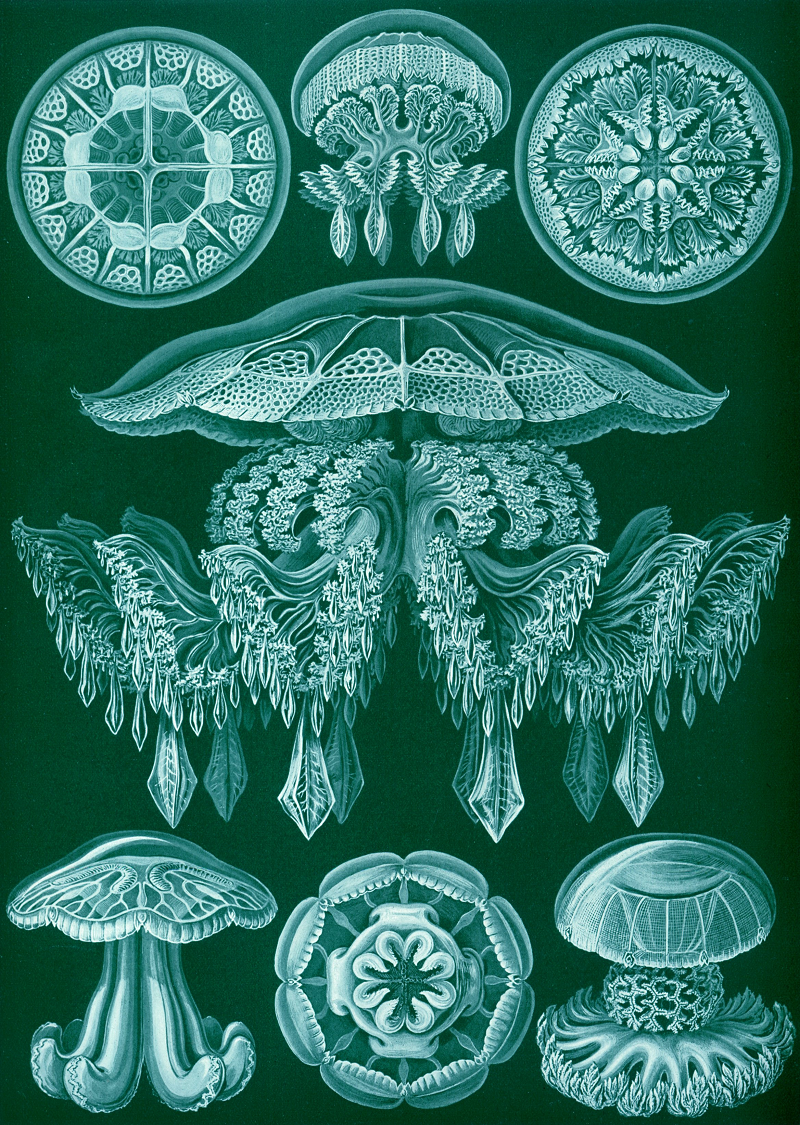
\includegraphics[width=\paperwidth]{CoverImage}}; % Background image
\draw[anchor=north] (midpoint) node [fill=white!30!white,fill opacity=0.8,text opacity=1,inner sep=1cm]{\Huge\centering\bfseries\sffamily\parbox[c][][t]{\paperwidth}
%
{\centering\huge Oracle Trace Files Explained\\[35pt] % Book title
{\Large Attempting to Document the Internals of an Oracle Trace File}\\[20pt] % Subtitle
{\huge Norman Dunbar}}}; % Author name
%
\end{tikzpicture}};
\end{tikzpicture}
\vfill
\endgroup

%----------------------------------------------------------------------------------------
%	COPYRIGHT PAGE
%----------------------------------------------------------------------------------------

\newpage
~\vfill
\thispagestyle{empty}

\noindent Copyright \copyright 2017,2018 Norman Dunbar\\ % Copyright notice

\noindent \textsc{Published by MeMyselfEye Publishing ;-)}\\ % Publisher

\noindent The latest version of the eBook can be downloaded from \href{https://github.com/NormanDunbar/OracleTraceFilesExplained}{the book's github repository}.\\ % URL

\noindent Licensed under the Creative Commons Attribution-NonCommercial 3.0 Unported License (the ``License''). You may not use this file except in compliance with the License. You may obtain a copy of the License at \url{http://creativecommons.org/licenses/by-nc/3.0}. Unless required by applicable law or agreed to in writing, software distributed under the License is distributed on an \textsc{``as is'' basis, without warranties or conditions of any kind}, either express or implied. See the License for the specific language governing permissions and limitations under the License.\\ % License information

\noindent \textit{First printing, July 2017} \\% Printing/edition date

%\noindent This pdf document was created on \textit{\pdfcreationdate}.

\noindent This pdf document was created on \textit{\the\day/\the\month/\the\year} at \textit{\DTMcurrenttime}.

%----------------------------------------------------------------------------------------
%	TABLE OF CONTENTS
%----------------------------------------------------------------------------------------

\chapterimage{ChapterImage} % Table of contents heading image

\pagestyle{empty} % No headers


\tableofcontents % Print the table of contents itself
\listoftables
%\listoffigures
\lstlistoflistings

\cleardoublepage % Forces the first chapter to start on an odd page so it's on the right

\pagestyle{fancy} % Print headers again

%----------------------------------------------------------------------------------------
%Here come the contents of the book...
%----------------------------------------------------------------------------------------
\mainmatter
% Define the chapter heading image to be used for all (subsequent) chapters.
\chapterimage{ChapterImage} % Chapter heading image

% Don't use these commands because using \mainmatter corrupts the
% index.
%\frontmatter

% The main meat of the book begins here.
%\mainmatter

\part{Oracle Trace Files}
\chapter{Introduction}\label{introduction}

Oracle trace files are not greatly documented. This document is an attempt to do so. It is \emph{not} official in any way and is based on a good few years of reading these files to help diagnose various database problems.

A trace file is really the best way to delve into what Oracle is doing, or to discover why something is taking so long - it shows you exactly what happened during the period that the session was being traced.

Even better, when you extract an Explain Plan from a trace file, it is showing you exactly how Oracle retrieved the data from the tables, and exactly where the time was spend in doing so. Running an \inline{Explain Plan for ...} statement in \emph{SQL*Plus}\program{SQL*Plus}, \emph{Toad}\program{Toad} etc tells you what Oracle \emph{might} do. The two are not always the same.

The trace files used (and abused) in this eBook were all self contained, and extracted from a dedicated session on the database. If you are using shared sessions, then you have the unfortunate problem of having bits of your session trace spread over any number of different trace files. Not fun.

From Oracle 10g onwards, a utility has been supplied, named \emph{trcsess}\program{Trcsess}. This allows you to collect together all the separate files and merge them into one, ready for analysis. Even better, it apparently can also merge Oracle 9i shared server session trace files. Bonus!

\section*{Trace File Extracts}

In the remainder of this eBook, extracts from trace files will be shown as follows:

\begin{lstlisting}[numbers=none]
WAIT #3220341128: nam='db file sequential read' ela= 1023 file#=3 block#=12 blocks=1 obj#=-1 tim=3520817183625
\end{lstlisting}

You will notice that long lines from the trace file are wrapped in the example above. However, all such wrapped lines are indicated by a \textbf{$\Longrightarrow$} at the start of the continuation line(s). Sometimes though, the break in the lines can be at an awkward position. Sadly, I can't help this, it's all automagically done and I have no input as to how, exactly, \LaTeX{} decides.

\section*{Code Listings}

SQL scripts (or any other program listings) will be listed as per the example below. The only difference being line numbers, in case I have to reference a particular point, and syntax highlighting.

\begin{lstlisting}[language=SQL]
select name, parameter1, parameter2, parameter3
from   v$event_name
where  name = 'db file sequential read';
\end{lstlisting}

\section*{Irregular Updates}

This eBook is a work in progress, I am always learning, or trying to. As I update it, the latest version will always appear on GitHub as detailed on the Copyright page above. Also on that page, you will be able to see the date and time that the version of the eBook you are reading, was generated. That's done automagically too, so I don't need to remember to update it - thankfully!

\section*{Comments}

Seen anything blatantly wrong? Something  you think needs a better explanation? Too many blatant plugs? You can either create an issue on GitHub, or, \href{mailto://norman@dunbar-it.co.uk}{email me} with details and I'll do my best to get it fixed.
\chapter{Oracle Trace Files Explained}\label{oracle-trace-files-explained}

\section{Trace File Sections}\label{trace-file-sections}

The trace file is made up of two main sections, the header and the trace details.

\subsection{The Header}\label{the-header}\index{Header, Trace File}\index{Trace File Header}

The header is the top of the file and consists of a few lines of text giving details of where the trace file came from, which server (operating System) it was created on, various details about the server and the database and so on.

The following is an example of a trace file created on a Windows server, running Oracle 11.2.0.4. Server, database and other potentially sensitive information has been obfuscated to protect the guilty, me!

\begin{lstlisting}[numbers=none,caption={Oracle 11g Trace File Header}]
Trace file C:\ORACLEDATABASE\diag\rdbms\cfg\cfg\trace\orcl_ora_27680_FREESPACE.trc
Oracle Database 11g Enterprise Edition Release 11.2.0.4.0 - 64bit Production
Windows NT Version V6.2  
CPU                 : 8 - type 8664, 8 Physical Cores
Process Affinity    : 0x0x0000000000000000
Memory (Avail/Total): Ph:29917M/57343M, Ph+PgF:24634M/65535M 
Instance name: orcl
Redo thread mounted by this instance: 1
Oracle process number: 373
Windows thread id: 27680, image: ORACLE.EXE (SHAD)


*** 2017-06-27 13:56:36.872
*** SESSION ID:(1017.1085) 2017-06-27 13:56:36.872
*** CLIENT ID:() 2017-06-27 13:56:36.872
*** SERVICE NAME:(ORCLSRV) 2017-06-27 13:56:36.872
*** MODULE NAME:(TOAD background query session) 2017-06-27 13:56:36.872
*** ACTION NAME:() 2017-06-27 13:56:36.872

=====================
\end{lstlisting}

The last line, consisting of equals signs, is the separator between the header and the following trace details.

In Oracle versions before 10g, the latter chunk of text is not found, the one detailing session, client, module etc, those first appeared at 10g.


\begin{note}
Sometimes, you might see a header that has a number of detail lines before the final separator, for example:

\begin{lstlisting}[numbers=none,caption={Oracle 11g Trace File Header - With Waits etc}]
...

*** 2017-05-08 12:39:13.496
*** SESSION ID:(777.2309) 2017-05-08 12:39:13.496
*** CLIENT ID:() 2017-05-08 12:39:13.496
*** SERVICE NAME:(SYS$USERS) 2017-05-08 12:39:13.496
*** MODULE NAME:(SQL*Plus) 2017-05-08 12:39:13.496
*** ACTION NAME:() 2017-05-08 12:39:13.496
 
WAIT #523653448: nam='SQL*Net message to client' ela= 1 driver id=1111838976 #bytes=1 p3=0 obj#=14232 tim=1743670562625
WAIT #523653448: nam='SQL*Net message from client' ela= 1027 driver id=1111838976 #bytes=1 p3=0 obj#=14232 tim=1743670564245
CLOSE #523653448:c=0,e=7,dep=0,type=1,tim=1743670564280
WAIT #0: nam='SQL*Net more data from client' ela= 12 driver id=1111838976 #bytes=10 p3=0 obj#=14232 tim=1743670564312
=====================
\end{lstlisting}

In this case, the trace was started after the session had parsed a query, and was in the process of executing it (\inline{EXEC} and, if necessary \inline{FETCH}) when the trace started. Oracle has not shown the \inline{PARSING IN CURSOR} line(s) for the query in question, which is a shame.

Normally, you can ignore the detail lines above the header separator, however, you sometimes see numerous \inline{WAIT} lines above the separator, in which case, there could be something to investigate. This is more likely to occur when you start tracing a session that is taking a huge amount of time, and is already under way when you begin the trace.
\end{note}



\subsection{Trace Details}\label{trace-details}

The majority of the trace file consists of the full trace details for the session that was traced. There are numerous lines of text here, each different, each with their own fields of one kind or another.

These are explained in the following sections.

\begin{note}
Remember, when Oracle writes a line to the trace file, it is done at the \emph{end} of the process that was indicated by the written line. For example, if you see a \inline{FETCH} line in the trace file, that was written at the time (\inline{tim}) that the \inline{FETCH} completed. The trace file should be considered a list of things \emph{that have happened} and not \emph{things that are about to happen}.
\end{note}

For example, a recent trace file that I had the pleasure of examining had over 2 million lines. The problem was to determine where a statement was losing over 2,000 seconds of time on its first \inline{EXEC} which it did not have on any of the subsequent \inline{EXEC}s.

The statement was parsed at \inline{dep=0} on line 36,656 but was not executed, again at \inline{dep=0} until line 284,530, as the following \texttt{grep} output shows:

\begin{lstlisting}[numbers=none,caption={Oracle 11g Problem Trace - \texttt{grep} output}]

grep -n "dep=0" tracefile.trc

...

36656:PARSE #11529215045668893824:c=0,e=1076,p=0,cr=0,cu=0,mis=1,r=0,dep=0,og=1,plh=0,tim=26375808573637

284530:EXEC #11529215045668893824:c=83870000,e=2048188431,p=1233,cr=45536,cu=18,mis=1,r=1,dep=0,og=1,plh=0,tim=26377856794348

...
\end{lstlisting}

From the above you can see that nothing took place between the \inline{PARSE} and the \inline{EXEC}, so any other SQL executed between those lines was done in order to facilitate the \inline{EXEC} at line 284,530. So that's where the time was lost, in recursive SQL statements, executed in order to carry out the required statement's \inline{EXEC}. 

A quick investigation showed that Oracle was gathering dynamic stats against numerous dictionary tables in the SYS schema, so after a quick \texttt{DBMS\_STATS.GATHER\_SCHEMA\_STATS} and a \texttt{DBMS\_STATS.GATHER\_DICTIONARY\_STATS} the lost time was restored and the problem went away.

We \emph{know} that the time was being lost in the \inline{EXEC} as the \inline{PARSE} of the statement had been written to the trace file at line 36,656 so at that point, the \inline{PARSE} had completed. The \inline{EXEC} did not complete until line 284,530, so everything between those lines was related to the \inline{EXEC} and nothing to do with the \inline{PARSE}.

Also, the \emph{elapsed time} for the \inline{EXEC} shows that the execution of the statement took 2048.188431 seconds (\emph{e=2048188431}).


\subsubsection{Timestamp Lines}\label{timestamp-lines}\index{Timestamps}

One line that you should be interested in is this one from the header above:

\begin{lstlisting}[numbers=none,caption={Time Stamp Line}]
*** 2017-06-27 13:56:36.872
\end{lstlisting}

This is the first timestamp line in the trace file and sets the baseline for all the \inline{tim} fields (these will be explained below) that follow, however, briefly, the \inline{tim} values are in microseconds (millionths of a second) from a specific ``epoch'' - which depends on the operating system - and there isn't a consistent, operating system independent, method of converting \inline{tim} values from a huge number of microseconds to an actual date and time that humans will understand.

There are usually a few timestamp lines written to the trace file, depending on how long it has been processing for, and these mean that we can, with a bit of fiddling, relate a \inline{tim} value to an actual time on the clock.

The \emph{first} \inline{tim} value that you see, following a timestamp line, will be the microsecond equivalent to the date and time in the timestamp line.

\subsubsection{Recursive SQL}\label{recursive-sql}\index{SQL!Recursive}\index{Recursive SQL}

Your SQL statements are normally executed as top-level statements, but Oracle might need to execute some (a lot!) of recursive SQL statements, in order that your statement can be processed. 

If, for example, you drop a user in a database with the \inline{drop user xxx cascade} statement, Oracle goes off and executes hundreds of separate SQL statement to find out what objects the user owns, or has privileges to, and undoes all of those before finally dropping the contents of the user and finally the user itself.

Top-level SQL\index{SQL!Top Level}\index{Top Level SQL} statements are identified by having a depth of zero. This can be seen in many of the trace file lines as \inline{dep=0} in the various lines of the trace file.

Recursive statements, executed in the background, have a depth greater than zero, and some of these require recursive statements of their own, and so on.

This recursion leads to a foible in the trace file, your statement appears last and all the possibly nested, recursive statements will normally appear first. This is simply because in order for your statement to be executed, the recursive statements have to run to completion \emph{first}.

For example, in a trace file I have open in front of me, the first statement with a \inline{dep=0} occurs at line 709 in the file. Everything prior to that runs at \inline{dep=3}, \inline{dep=2} or \inline{dep=1} and complete before I can see my own SQL statement. 

Under normal circumstances, a statement that is parsed (executed etc) at \inline{dep=$n$}, where $n > 0$, has been called recursively, to facilitate a statement, that will follow in the trace file, that is itself parsed (executed etc) at \inline{dep=$n-1$}.

\subsubsection{Waits}\label{waits}\index{Waits}

\inline{WAIT} lines in a trace file are similar, in that the \inline{WAIT} must complete, and so is written to the trace file, \emph{before} the statement that incurred the wait. For example, a \inline{FETCH} that had to wait for \inline{db file scattered read} events, will appear later in the trace file that the individual \inline{WAIT} lines that the \inline{FETCH} suffered from.

\subsubsection{Cursor Ids}\label{cursor-ids}\index{Cursor IDs}

Every time you see a `\#' followed by a number, you are looking at a cursor ID. In previous versions of Oracle, these were simply an ever increasing number, starting from 1 and increasing by 1 for each new cursor.

In Oracle 11g, the cursor \emph{appears} to be an address in memory\footnote{But don't quote me on this, I saw it written down somewhere on the Oracle Support web site, but now that I need it, I cannot find it again. Sigh!}, and \emph{will be reused} as cursors are closed and new ones opened. You cannot assume, therefore, that a cursor with a specific ID at the end of the trace file, relates to any other lines with that same ID previously written to the trace file, without checking for any intervening \inline{CLOSE} lines with the same ID - that's just how it is now!

\subsubsection{Active or Inactive}\label{active-or-inactive}

You might want to look in the \inline{STATUS} column in \inline{V\$SESSION} to determine if the session is active - doing \emph{something} - or not. However, you must be aware that the \inline{STATUS} column only gives an active reading when the statement is in a \inline{PARSE}, \inline{EXEC} or \inline{FETCH} phase of execution. If the statement is in a \inline{WAIT}, for example, it will show as inactive - but it is actually still processing the current statement. Something to bear in mind.

\section{Trace File Details}\label{trace-file-details}

As mentioned above, the trace file details, which consists of many different entries, is discussed in the following chapter.

\chapter{Trace File Entries}

\section{PARSING IN CURSOR}\label{parsing-in-cursor}\index{Parsing in Cursor}

This is \emph{usually} the first line you will see for a cursor. It shows the full SQL statement between the \inline{PARSING IN CURSOR} line and the \inline{END OF STMT} line. The SQL is displayed exactly as the user (or application) entered it. However, if the statement is invalid, or cannot be parsed, you will not see this, or the \inline{PARSE} line in the trace file, you will only see a \inline{PARSE ERROR} line instead.

This is not the actual \inline{PARSE} for the cursor though, that normally follows on later, usually!

As an example, here is the \inline{PARSING IN CURSOR} line for the SQL query that Toad runs in the background to extract the free space used in the database by various tablespaces, including temporary ones. However, I'm not showing the SQL here:

\begin{lstlisting}[numbers=none,caption={Parsing In Cursor Line}]
PARSING IN CURSOR #3220341128 len=3081 dep=0 uid=0 oct=3 lid=0 tim=3520788574727 hv=3219027813 ad='7ffcb6778350' sqlid='7bwtj5azxwxv5'
\end{lstlisting}

The various fields defined, and their descriptions can be seen in the table below.

\begin{longtable}[]{@{}l|l@{}}
\hline
\caption{Parsing in Cursor - Fields\ldots{}\textit{continues on next page}}
\endfoot
\caption{Parsing in Cursor - Fields}
\endlastfoot

\toprule
\begin{minipage}[b]{0.14\columnwidth}\raggedright\strut
Code\strut
\end{minipage} & \begin{minipage}[b]{0.65\columnwidth}\raggedright\strut
Description\strut
\end{minipage}\tabularnewline
\midrule
\endhead
\begin{minipage}[t]{0.14\columnwidth}\raggedright\strut
\#nnnn\strut
\end{minipage} & \begin{minipage}[t]{0.65\columnwidth}\raggedright\strut
The cursor ID. This may be reused if for future cursors if this one is
closed, and another opened.\strut
\end{minipage}\tabularnewline
\begin{minipage}[t]{0.14\columnwidth}\raggedright\strut
len\strut
\end{minipage} & \begin{minipage}[t]{0.65\columnwidth}\raggedright\strut
The size, in bytes? Characters? of the SQL statement.\strut
\end{minipage}\tabularnewline
\begin{minipage}[t]{0.14\columnwidth}\raggedright\strut
dep\strut
\end{minipage} & \begin{minipage}[t]{0.65\columnwidth}\raggedright\strut
Recursion level. 0 = Top-level, user, SQL.\strut
\end{minipage}\tabularnewline
\begin{minipage}[t]{0.14\columnwidth}\raggedright\strut
uid\strut
\end{minipage} & \begin{minipage}[t]{0.65\columnwidth}\raggedright\strut
The user id of the user parsing the statement.\strut
\end{minipage}\tabularnewline
\begin{minipage}[t]{0.14\columnwidth}\raggedright\strut
oct\strut
\end{minipage} & \begin{minipage}[t]{0.65\columnwidth}\raggedright\strut
Oracle Command Code of the SQL Statement. (See Appendices.)\strut
\end{minipage}\tabularnewline
\begin{minipage}[t]{0.14\columnwidth}\raggedright\strut
lid\strut
\end{minipage} & \begin{minipage}[t]{0.65\columnwidth}\raggedright\strut
Unknown - perhaps the proxy login ID?\strut
\end{minipage}\tabularnewline
\begin{minipage}[t]{0.14\columnwidth}\raggedright\strut
tim\strut
\end{minipage} & \begin{minipage}[t]{0.65\columnwidth}\raggedright\strut
Time, in microseconds, that the details were written out to the trace file.\strut
\end{minipage}\tabularnewline
\begin{minipage}[t]{0.14\columnwidth}\raggedright\strut
hv\strut
\end{minipage} & \begin{minipage}[t]{0.65\columnwidth}\raggedright\strut
Hash Value for the statement.\strut
\end{minipage}\tabularnewline
\begin{minipage}[t]{0.14\columnwidth}\raggedright\strut
ad\strut
\end{minipage} & \begin{minipage}[t]{0.65\columnwidth}\raggedright\strut
Cursor address in memory?\strut
\end{minipage}\tabularnewline
\begin{minipage}[t]{0.14\columnwidth}\raggedright\strut
sqlid\strut
\end{minipage} & \begin{minipage}[t]{0.65\columnwidth}\raggedright\strut
The SQL ID for the statement.\strut
\end{minipage}\tabularnewline
\bottomrule
\end{longtable}

The \inline{uid} field references the column \inline{USER\_ID} in the views \inline{DBA\_USERS}, \inline{ALL\_USERS} and \inline{USER\_USERS}.

The \inline{lid} field is unknown at present. It's probably an ID of some kind, but for what? Perhaps it is something to do with proxy logins and \inline{lid} is the login identifier?

As mentioned, the cursor ID field has a value that may (or may not) be an address in memory. However, that's not the same as the \inline{ad} field, which is (I think) an address in memory for the cursor.

The \inline{sqlid} field is the same as the \inline{SQL\_ID} column in \inline{V\$SQL}. The \inline{hv} field is the hash value that Oracle used to determine if this statement was to be found in the cache or not. It matches the \inline{SQL\_HASH\_VALUE} (and \inline{PREV\_HASH\_VALUE}) column in \inline{V\$SESSION} and also the \inline{HASH\_VALUE} column in \inline{V\$SQL}.

Sometime Oracle will not write these lines to the trace file. If the cursor has been parsed, and subsequently closed, then re-parsed, you will see a \inline{PARSE} line but not a new \inline{PARSING IN CURSOR} for the statement. This \emph{appears} to be only on those occasions where the statement is re-parsed \emph{immediately} after being closed. I have not seen this ``feature'' when the cursor ID was used by a different statement in between.

\newpage\section{PARSE}\label{parse}\traceline{PARSE}

Normally, after the \inline{PARSING IN CURSOR} lines, you will see a \inline{PARSE} line for the same cursor ID. This is not always the case, for example, if you started the trace after the statement had been parsed, Oracle *may* write the \inline{PARSING IN CURSOR} lines, but not the \inline{PARSE}, to the trace file.

Other times when the \inline{PARSE} line will not be seen is when the cursor associated with the SQL statement was previously \inline{CLOSE}d but Oracle decided not to hard close the cursor but instead cached it for future use. Normally this happens if \inline{SESSION\_CACHED\_CURSORS} is non-zero and the SQL statement has already been \inline{PARSE}d at least three times.

See the \inline{type} parameter for the \inline{CLOSE} trace line in Section~\ref{close} on Page~\pageref{close} for details of how and when a cursor \emph{might} be cached.

A typical \inline{PARSE} line will look like this:

\begin{lstlisting}[numbers=none,caption={Parse Line}]
PARSE #491311368:c=0,e=452,p=0,cr=0,cu=0,mis=1,r=0,dep=0,og=1,plh=1388734953,tim=97734887542
\end{lstlisting}

\begin{longtable}[]{@{}l|l@{}}
\hline
\caption{Parse - Fields\ldots{}\textit{continues on next page}}
\endfoot
\caption{Parse - Fields}
\endlastfoot

\toprule
\begin{minipage}[b]{0.14\columnwidth}\raggedright\strut
Code\strut
\end{minipage} & \begin{minipage}[b]{0.65\columnwidth}\raggedright\strut
Description\strut
\end{minipage}\tabularnewline
\midrule
\endhead
\begin{minipage}[t]{0.14\columnwidth}\raggedright\strut
\#nnnn\strut
\end{minipage} & \begin{minipage}[t]{0.65\columnwidth}\raggedright\strut
The cursor ID. This may be reused if for future cursors if this one is
closed, and another opened.\strut
\end{minipage}\tabularnewline
\begin{minipage}[t]{0.14\columnwidth}\raggedright\strut
c\strut
\end{minipage} & \begin{minipage}[t]{0.65\columnwidth}\raggedright\strut
Elapsed CPU time. Microseconds.\strut
\end{minipage}\tabularnewline
\begin{minipage}[t]{0.14\columnwidth}\raggedright\strut
e\strut
\end{minipage} & \begin{minipage}[t]{0.65\columnwidth}\raggedright\strut
Elapsed wall clock time, also in microseconds.\strut
\end{minipage}\tabularnewline
\begin{minipage}[t]{0.14\columnwidth}\raggedright\strut
p\strut
\end{minipage} & \begin{minipage}[t]{0.65\columnwidth}\raggedright\strut
The number of physical reads (blocks) that were necessary in order to
carry out this \inline{PARSE}.\strut
\end{minipage}\tabularnewline
\begin{minipage}[t]{0.14\columnwidth}\raggedright\strut
cr\strut
\end{minipage} & \begin{minipage}[t]{0.65\columnwidth}\raggedright\strut
The number of consistent reads (blocks) that were necessary in order to
carry out this \inline{PARSE}.\strut
\end{minipage}\tabularnewline
\begin{minipage}[t]{0.14\columnwidth}\raggedright\strut
cu\strut
\end{minipage} & \begin{minipage}[t]{0.65\columnwidth}\raggedright\strut
The number of current reads (blocks) that were necessary in order to
carry out this \inline{PARSE}.\strut
\end{minipage}\tabularnewline
\begin{minipage}[t]{0.14\columnwidth}\raggedright\strut
mis\strut
\end{minipage} & \begin{minipage}[t]{0.65\columnwidth}\raggedright\strut
Whether this statement was found in the cache (0) or not (1). Indicates
whether or not a hard parse was required. Seeing a 1 is bad,
usually.\strut
\end{minipage}\tabularnewline
\begin{minipage}[t]{0.14\columnwidth}\raggedright\strut
r\strut
\end{minipage} & \begin{minipage}[t]{0.65\columnwidth}\raggedright\strut
Rows processed.\strut
\end{minipage}\tabularnewline
\begin{minipage}[t]{0.14\columnwidth}\raggedright\strut
dep\strut
\end{minipage} & \begin{minipage}[t]{0.65\columnwidth}\raggedright\strut
Recursion level. 0 = Top-level, user, SQL.\strut
\end{minipage}\tabularnewline
\begin{minipage}[t]{0.14\columnwidth}\raggedright\strut
og\strut
\end{minipage} & \begin{minipage}[t]{0.65\columnwidth}\raggedright\strut
Optimiser goal. 1 = ALL\_ROWS, 2 = FIRST\_ROWS, 3 = RULE, 4 = CHOOSE.
Depending on your version of Oracle, you may not see some of the
above.\strut
\end{minipage}\tabularnewline
\begin{minipage}[t]{0.14\columnwidth}\raggedright\strut
plh\strut
\end{minipage} & \begin{minipage}[t]{0.65\columnwidth}\raggedright\strut
Execution plan hash value.\strut
\end{minipage}\tabularnewline
\begin{minipage}[t]{0.14\columnwidth}\raggedright\strut
tim\strut
\end{minipage} & \begin{minipage}[t]{0.65\columnwidth}\raggedright\strut
Time, in microseconds, when the parse for the statement completed.
\textbf{Not} the time it took.\strut
\end{minipage}\tabularnewline
\bottomrule
\end{longtable}

The \inline{plh} value is a value that corresponds to the column \inline{PLAN\_HASH\_VALUE} in \inline{V\$SQL\_PLAN}, \inline{V\$SQL\_PLAN\_STATISTICS\_ALL} and \inline{V\$SQLSTATS}. (There may be other views where this value appears, depending on the Oracle version in use.)

\subsection*{Block Details}\label{block-details}

\index{Block Details!Physical blocks}
\index{Block Details!Current blocks}
\index{Block Details!Consistent blocks}

The \inline{p}, \inline{cr} and \inline{cu} statistics are the usual ones for block reads, viz:

\begin{itemize}
\tightlist
\item
  Physical reads occur when Oracle must read a block, from disc, into   the buffer cache. This indicates also an additional \inline{cu} as the block will be used unchanged.
\item
  Consistent reads are the number of blocks of UNDO that Oracle applied   to one or more blocks, in order to return the data in those blocks, to   the state they were in when the ``query'' started. The query in this   case, would be any or all recursive queries necessary to facilitate   the \inline{PARSE}.
\item
  Current Reads are blocks that Oracle used without needing to roll them   back to the start of the ``query''.
\end{itemize}

The fields for an \inline{PARSE} are the same as those for an \inline{EXEC} and a \inline{FETCH} - see below.

The \inline{r} field is \emph{interesting}. Surely only a \inline{FETCH} would process some rows? I thought so too, and in all the trace files I've come across, I have yet to see (ok, yet to \emph{notice}) a \inline{PARSE} line with anything other than \inline{r=0}. I wonder why Oracle have it as part of the \inline{PARSE}? Maybe, because they use the same format of line for the \inline{PARSE} and \inline{EXEC} they decided just to use the same one, and set the row count for a \inline{PARSE} to zero?\footnote{We may never know!}

\newpage\section{PARSE ERROR}\label{parse-error}\traceline{PARSE ERROR}

If a \inline{PARSE} goes wrong for some reason, the trace file will show something like the following:

\begin{lstlisting}[numbers=none,caption={Parse Error Line}]
PARSE ERROR #491311368:len=26 dep=0 uid=755 oct=3 lid=755 tim=97734836031 err=1031
SELECT LIVE_DEV FROM SITE
\end{lstlisting}

There will not normally be a \inline{PARSING IN CURSOR} or a \inline{PARSE} shown in the trace file for this statement.

\begin{longtable}[]{@{}l|l@{}}
\hline
\caption{Parse Error - Fields\ldots{}\textit{continues on next page}}
\endfoot
\caption{Parse Error - Fields}
\endlastfoot

\toprule
\begin{minipage}[b]{0.14\columnwidth}\raggedright\strut
Code\strut
\end{minipage} & \begin{minipage}[b]{0.65\columnwidth}\raggedright\strut
Description\strut
\end{minipage}\tabularnewline
\midrule
\endhead
\begin{minipage}[t]{0.14\columnwidth}\raggedright\strut
\#nnnn\strut
\end{minipage} & \begin{minipage}[t]{0.65\columnwidth}\raggedright\strut
The cursor ID. This may be reused if for future cursors if this one is
closed, and another opened.\strut
\end{minipage}\tabularnewline
\begin{minipage}[t]{0.14\columnwidth}\raggedright\strut
len\strut
\end{minipage} & \begin{minipage}[t]{0.65\columnwidth}\raggedright\strut
The length of the SQL statement in bytes, maybe characters depending on
your characterset.\strut
\end{minipage}\tabularnewline
\begin{minipage}[t]{0.14\columnwidth}\raggedright\strut
dep\strut
\end{minipage} & \begin{minipage}[t]{0.65\columnwidth}\raggedright\strut
Recursion level. 0 = Top-level, user, SQL.\strut
\end{minipage}\tabularnewline
\begin{minipage}[t]{0.14\columnwidth}\raggedright\strut
uid\strut
\end{minipage} & \begin{minipage}[t]{0.65\columnwidth}\raggedright\strut
The user id of the user parsing the statement.\strut
\end{minipage}\tabularnewline
\begin{minipage}[t]{0.14\columnwidth}\raggedright\strut
oct\strut
\end{minipage} & \begin{minipage}[t]{0.65\columnwidth}\raggedright\strut
Oracle Command Code of the SQL Statement. (See Appendices.)\strut
\end{minipage}\tabularnewline
\begin{minipage}[t]{0.14\columnwidth}\raggedright\strut
lid\strut
\end{minipage} & \begin{minipage}[t]{0.65\columnwidth}\raggedright\strut
Unknown - perhaps Login ID for proxy logins?\strut
\end{minipage}\tabularnewline
\begin{minipage}[t]{0.14\columnwidth}\raggedright\strut
tim\strut
\end{minipage} & \begin{minipage}[t]{0.65\columnwidth}\raggedright\strut
Time, in microseconds, when this parse error was detected.\strut
\end{minipage}\tabularnewline
\begin{minipage}[t]{0.14\columnwidth}\raggedright\strut
err\strut
\end{minipage} & \begin{minipage}[t]{0.65\columnwidth}\raggedright\strut
The Oracle error code that caused the parse to fail.\strut
\end{minipage}\tabularnewline
\bottomrule
\end{longtable}

In this case, there was an error \inline{ORA-01031: insufficient privileges} as the user parsing the statement did not have the required privileges to see the table in question.

The \inline{uid} field references the column \inline{USER\_ID} in the views \inline{DBA\_USERS}, \inline{ALL\_USERS} and \inline{USER\_USERS}.

\newpage\section{EXEC}\label{exec}\traceline{EXEC}

The \inline{EXEC} phase of a statement's execution is when Oracle dives into the database to build a result set of the desired data. It need not be the complete result set though, so beware of that.

A typical \inline{EXEC} will resemble the following:

\begin{lstlisting}[numbers=none,caption={Exec Line}]
EXEC #3220341128:c=0,e=101,p=0,cr=0,cu=0,mis=0,r=0,dep=0,og=1,plh=2215247290,tim=3520788606189
\end{lstlisting}

Bear in mind, however, that the \inline{EXEC} elapsed times do not necessarily bear any resemblance to the entire time it took for the user to get a response. That response time includes the \inline{PARSE}, \inline{EXEC}, all the \inline{FETCH}es and all the \inline{WAIT}s that were encountered.

The fields in an \inline{EXEC} are as follows:

\begin{longtable}[]{@{}l|l@{}}
\hline
\caption{Exec - Fields\ldots{}\textit{continues on next page}}
\endfoot
\caption{Exec - Fields}
\endlastfoot

\toprule
\begin{minipage}[b]{0.14\columnwidth}\raggedright\strut
Code\strut
\end{minipage} & \begin{minipage}[b]{0.65\columnwidth}\raggedright\strut
Description\strut
\end{minipage}\tabularnewline
\midrule
\endhead
\begin{minipage}[t]{0.14\columnwidth}\raggedright\strut
\#nnnn\strut
\end{minipage} & \begin{minipage}[t]{0.65\columnwidth}\raggedright\strut
The cursor ID. This may be reused if for future cursors if this one is
closed, and another opened.\strut
\end{minipage}\tabularnewline
\begin{minipage}[t]{0.14\columnwidth}\raggedright\strut
c\strut
\end{minipage} & \begin{minipage}[t]{0.65\columnwidth}\raggedright\strut
Elapsed CPU time. Microseconds.\strut
\end{minipage}\tabularnewline
\begin{minipage}[t]{0.14\columnwidth}\raggedright\strut
e\strut
\end{minipage} & \begin{minipage}[t]{0.65\columnwidth}\raggedright\strut
Elapsed wall clock time, also in microseconds.\strut
\end{minipage}\tabularnewline
\begin{minipage}[t]{0.14\columnwidth}\raggedright\strut
p\strut
\end{minipage} & \begin{minipage}[t]{0.65\columnwidth}\raggedright\strut
The number of physical reads (blocks) that were necessary in order to
carry out this \inline{PARSE}.\strut
\end{minipage}\tabularnewline
\begin{minipage}[t]{0.14\columnwidth}\raggedright\strut
cr\strut
\end{minipage} & \begin{minipage}[t]{0.65\columnwidth}\raggedright\strut
The number of consistent reads (blocks) that were necessary in order to
carry out this \inline{PARSE}.\strut
\end{minipage}\tabularnewline
\begin{minipage}[t]{0.14\columnwidth}\raggedright\strut
cu\strut
\end{minipage} & \begin{minipage}[t]{0.65\columnwidth}\raggedright\strut
The number of current reads (blocks) that were necessary in order to
carry out this \inline{PARSE}.\strut
\end{minipage}\tabularnewline
\begin{minipage}[t]{0.14\columnwidth}\raggedright\strut
mis\strut
\end{minipage} & \begin{minipage}[t]{0.65\columnwidth}\raggedright\strut
Whether this statement was found in the cache (0) or not (1). Indicates
whether or not a hard parse was required. Seeing a 1 is bad,
usually.\strut
\end{minipage}\tabularnewline
\begin{minipage}[t]{0.14\columnwidth}\raggedright\strut
dep\strut
\end{minipage} & \begin{minipage}[t]{0.65\columnwidth}\raggedright\strut
Recursion level. 0 = Top-level, user, SQL.\strut
\end{minipage}\tabularnewline
\begin{minipage}[t]{0.14\columnwidth}\raggedright\strut
r\strut
\end{minipage} & \begin{minipage}[t]{0.65\columnwidth}\raggedright\strut
Rows processed.\strut
\end{minipage}\tabularnewline
\begin{minipage}[t]{0.14\columnwidth}\raggedright\strut
og\strut
\end{minipage} & \begin{minipage}[t]{0.65\columnwidth}\raggedright\strut
Optimiser goal. 1 = ALL\_ROWS, 2 = FIRST\_ROWS, 3 = RULE, 4 = CHOOSE.
Depending on your version of Oracle, you may not see some of the
above.\strut
\end{minipage}\tabularnewline
\begin{minipage}[t]{0.14\columnwidth}\raggedright\strut
plh\strut
\end{minipage} & \begin{minipage}[t]{0.65\columnwidth}\raggedright\strut
Execution plan hash value.\strut
\end{minipage}\tabularnewline
\begin{minipage}[t]{0.14\columnwidth}\raggedright\strut
tim\strut
\end{minipage} & \begin{minipage}[t]{0.65\columnwidth}\raggedright\strut
Time, in microseconds, at which this \inline{EXEC} statement was completed.\strut
\end{minipage}\tabularnewline
\bottomrule
\end{longtable}

The fields for an \inline{EXEC} are the same as those for a \inline{PARSE} (and \inline{FETCH} - see below).

The \inline{r} field is \emph{interesting}. Surely only a \inline{FETCH} would process some rows? Not necessarily. Normally, when \inline{EXEC}ing a statement, the number of rows processed is indeed zero, but some PL/SQL, for example, returns a row count of 1. In my demonstration trace file I see 4 statements whose \inline{EXEC} has \inline{r=1} and all of them are of the format:

\begin{lstlisting}[caption={PL/SQL Exec Example}]
begin
    do_something();
end;
\end{lstlisting}

The ``do\_something()'' call is to \inline{DBMS\_MONITOR.START\_TRACE}, \inline{DBMS\_MONITOR.STOP\_TRACE} and calls to \inline{DBMS\_OUTPUT.GET\_LINE}. These statements have no \inline{FETCH} calls.

You may wish to refer back to page \pageref{block-details} for details of the \inline{p}, \inline{cr} and \inline{cu} block statistics in the \inline{EXEC} line.

\newpage\section{FETCH}\label{fetch}\traceline{FETCH}

After processing the \inline{EXEC} call, and any associated \inline{WAIT}s, Oracle may \inline{FETCH} some, or all, of the rows returned by the query. A \inline{FETCH} line may resemble the following:

\begin{lstlisting}[numbers=none,caption={Fetch Line}]
FETCH #3220341128:c=1812500,e=28665431,p=11137,cr=50774,cu=316,mis=0,r=30,dep=0,og=1,plh=2215247290,tim=3520817271640
\end{lstlisting}

And anyone paying close attention will notice that the time it took to \inline{FETCH} 30 rows was a little excessive at 28.66 seconds. In case you are wondering, this is a query against \inline{DBA\_FREE\_SPACE} on an 11.2.0.4 database, and it is taking so long as it is hitting the \emph{never to be solved} \href{https://support.oracle.com/epmos/faces/BugDisplay?_afrLoop=109163696075238\&id=19125876\&_afrWindowMode=0\&_adf.ctrl-state=9eq93xdtt_165}{Bug 19125876} which affects 11.20.4 on AIX on Power Systems. Unfortunately, \emph{this} trace file is from a Windows server. The bug was logged on 30th June 2014, last updated on 26th June 2017, \emph{and is not yet fixed!}

\begin{longtable}[]{@{}l|l@{}}
\hline
\caption{Fetch - Fields\ldots{}\textit{continues on next page}}
\endfoot
\caption{fetch - Fields}
\endlastfoot

\toprule
\begin{minipage}[b]{0.14\columnwidth}\raggedright\strut
Code\strut
\end{minipage} & \begin{minipage}[b]{0.65\columnwidth}\raggedright\strut
Description\strut
\end{minipage}\tabularnewline
\midrule
\endhead
\begin{minipage}[t]{0.14\columnwidth}\raggedright\strut
\#nnnn\strut
\end{minipage} & \begin{minipage}[t]{0.65\columnwidth}\raggedright\strut
The cursor ID. This may be reused if for future cursors if this one is
closed, and another opened.\strut
\end{minipage}\tabularnewline
\begin{minipage}[t]{0.14\columnwidth}\raggedright\strut
c\strut
\end{minipage} & \begin{minipage}[t]{0.65\columnwidth}\raggedright\strut
Elapsed CPU time. Microseconds.\strut
\end{minipage}\tabularnewline
\begin{minipage}[t]{0.14\columnwidth}\raggedright\strut
e\strut
\end{minipage} & \begin{minipage}[t]{0.65\columnwidth}\raggedright\strut
Elapsed wall clock time, also in microseconds.\strut
\end{minipage}\tabularnewline
\begin{minipage}[t]{0.14\columnwidth}\raggedright\strut
p\strut
\end{minipage} & \begin{minipage}[t]{0.65\columnwidth}\raggedright\strut
The number of physical reads (blocks) that were necessary in order to
carry out this \inline{FETCH}.\strut
\end{minipage}\tabularnewline
\begin{minipage}[t]{0.14\columnwidth}\raggedright\strut
cr\strut
\end{minipage} & \begin{minipage}[t]{0.65\columnwidth}\raggedright\strut
The number of consistent reads (blocks) that were necessary in order to
carry out this \inline{FETCH}.\strut
\end{minipage}\tabularnewline
\begin{minipage}[t]{0.14\columnwidth}\raggedright\strut
cu\strut
\end{minipage} & \begin{minipage}[t]{0.65\columnwidth}\raggedright\strut
The number of current reads (blocks) that were necessary in order to
carry out this \inline{FETCH}.\strut
\end{minipage}\tabularnewline
\begin{minipage}[t]{0.14\columnwidth}\raggedright\strut
mis\strut
\end{minipage} & \begin{minipage}[t]{0.65\columnwidth}\raggedright\strut
Whether this statement was found in the cache (0) or not (1).\strut
\end{minipage}\tabularnewline
\begin{minipage}[t]{0.14\columnwidth}\raggedright\strut
r\strut
\end{minipage} & \begin{minipage}[t]{0.65\columnwidth}\raggedright\strut
Rows processed.\strut
\end{minipage}\tabularnewline
\begin{minipage}[t]{0.14\columnwidth}\raggedright\strut
dep\strut
\end{minipage} & \begin{minipage}[t]{0.65\columnwidth}\raggedright\strut
Recursion level. 0 = Top-level, user, SQL.\strut
\end{minipage}\tabularnewline
\begin{minipage}[t]{0.14\columnwidth}\raggedright\strut
og\strut
\end{minipage} & \begin{minipage}[t]{0.65\columnwidth}\raggedright\strut
Optimiser goal. 1 = ALL\_ROWS, 2 = FIRST\_ROWS, 3 = RULE, 4 = CHOOSE.
Depending on your version of Oracle, you may not see some of the
above.\strut
\end{minipage}\tabularnewline
\begin{minipage}[t]{0.14\columnwidth}\raggedright\strut
plh\strut
\end{minipage} & \begin{minipage}[t]{0.65\columnwidth}\raggedright\strut
Execution plan hash value.\strut
\end{minipage}\tabularnewline
\begin{minipage}[t]{0.14\columnwidth}\raggedright\strut
tim\strut
\end{minipage} & \begin{minipage}[t]{0.65\columnwidth}\raggedright\strut
Time, in microseconds, that this one fetch was completed.\strut
\end{minipage}\tabularnewline
\bottomrule
\end{longtable}

The fields for a \inline{FETCH} are also the same as those for a \inline{PARSE} and \inline{EXEC}.

The \inline{mis} field is \emph{interesting}. Surely only a \inline{PARSE} would indicate a miss in the cache? Again, I think Oracle are using the same format of a trace line for \inline{PARSE}, \inline{EXEC} and \inline{FETCH} and simply ignoring or defaulting certain, non-applicable, fields.

You may wish to refer back to page \pageref{block-details} for details of the \inline{p}, \inline{cr} and \inline{cu} block statistics in the \inline{EXEC} line.

\newpage\section{WAIT}\label{wait}\traceline{WAIT}

This is the meat of the trace file, usually. Under normal circumstances, it's usual for the various phases of execution (\inline{PARSE}, \inline{EXEC} and \inline{FETCH}) to encounter some \inline{WAIT} events. And I would say, personally\footnote{Beware of   small sample sizes!}, that these \inline{WAIT} states are where the vast majority of the total response time is encountered.

A \inline{WAIT} line in the trace file will resemble the following example, up until Oracle 9i at the latest:

\begin{lstlisting}[numbers=none,caption={Wait Line - Oracle 9i}]
WAIT #3220341128: nam='db file sequential read' ela= 2769 p1=37 p2=12931 p3=1
\end{lstlisting}

\begin{longtable}[]{@{}l|l@{}}
\hline
\caption{Wait - Fields for Oracle 9i\ldots{}\textit{continues on next page}}
\endfoot
\caption{Wait - Fields for Oracle 9i}
\endlastfoot

\toprule
\begin{minipage}[b]{0.14\columnwidth}\raggedright\strut
Code\strut
\end{minipage} & \begin{minipage}[b]{0.65\columnwidth}\raggedright\strut
Description\strut
\end{minipage}\tabularnewline
\midrule
\endhead
\begin{minipage}[t]{0.14\columnwidth}\raggedright\strut
\#nnnn\strut
\end{minipage} & \begin{minipage}[t]{0.65\columnwidth}\raggedright\strut
The cursor ID. This may be reused if for future cursors if this one is
closed, and another opened.\strut
\end{minipage}\tabularnewline
\begin{minipage}[t]{0.14\columnwidth}\raggedright\strut
nam\strut
\end{minipage} & \begin{minipage}[t]{0.65\columnwidth}\raggedright\strut
The name of the wait event encountered.\strut
\end{minipage}\tabularnewline
\begin{minipage}[t]{0.14\columnwidth}\raggedright\strut
ela\strut
\end{minipage} & \begin{minipage}[t]{0.65\columnwidth}\raggedright\strut
Elapsed wall clock time, in microseconds.\strut
\end{minipage}\tabularnewline
\begin{minipage}[t]{0.14\columnwidth}\raggedright\strut
p1\strut
\end{minipage} & \begin{minipage}[t]{0.65\columnwidth}\raggedright\strut
Event parameter 1.\strut
\end{minipage}\tabularnewline
\begin{minipage}[t]{0.14\columnwidth}\raggedright\strut
p2\strut
\end{minipage} & \begin{minipage}[t]{0.65\columnwidth}\raggedright\strut
Event parameter 2.\strut
\end{minipage}\tabularnewline
\begin{minipage}[t]{0.14\columnwidth}\raggedright\strut
p3\strut
\end{minipage} & \begin{minipage}[t]{0.65\columnwidth}\raggedright\strut
Event parameter 3.\strut
\end{minipage}\tabularnewline
\bottomrule
\end{longtable}

The \inline{p1}, \inline{p2} and \inline{p3} parameters are different depending on the wait event name. You may require to look them up in \inline{V\$EVENT\_NAME} to understand what they refer to. For the event above, we see the following:

\begin{itemize}
\tightlist
\item
  p1 is the file number;
\item
  p2 is the (starting) block number;
\item
  p3 is the number of blocks requested.
\end{itemize}

You may wish to use the following query to determine the various parameters for the \inline{WAIT} events seen in the trace file:

\begin{lstlisting}[language=SQL,caption={Extracting Event Names for Oracle 9i}]
select name, parameter1, parameter2, parameter3
from   v$event_name
where  name = 'db file sequential read';
\end{lstlisting}

Substitute the appropriate event name for your particular \inline{WAIT} event of course. And, don't forget, it \emph{is} case sensitive - Oracle are seriously inconsistent when it comes to naming events!

In Oracle versions 10g onwards, the format is much easier to understand as the generic \inline{p1}, \inline{p2} and \inline{p3} have been replaced by something more meaningful, as follows for the same \inline{WAIT} event:

\begin{lstlisting}[numbers=none,caption={Wait Line - Oracle 10g Onwards}]
WAIT #3220341128: nam='db file sequential read' ela= 1023 file#=3 block#=12 blocks=1 obj#=-1 tim=3520817183625
\end{lstlisting}

\begin{longtable}[]{@{}l|l@{}}
\hline
\caption{Parse - Fields for Oracle 10g Onwards\ldots{}\textit{continues on next page}}
\endfoot
\caption{Parse - Fields for Oracle 10g Onwards}
\endlastfoot

\toprule
\begin{minipage}[b]{0.14\columnwidth}\raggedright\strut
Code\strut
\end{minipage} & \begin{minipage}[b]{0.65\columnwidth}\raggedright\strut
Description\strut
\end{minipage}\tabularnewline
\midrule
\endhead
\begin{minipage}[t]{0.14\columnwidth}\raggedright\strut
\#nnnn\strut
\end{minipage} & \begin{minipage}[t]{0.65\columnwidth}\raggedright\strut
The cursor ID. This may be reused if for future cursors if this one is
closed, and another opened.\strut
\end{minipage}\tabularnewline
\begin{minipage}[t]{0.14\columnwidth}\raggedright\strut
nam\strut
\end{minipage} & \begin{minipage}[t]{0.65\columnwidth}\raggedright\strut
The name of the wait event encountered.\strut
\end{minipage}\tabularnewline
\begin{minipage}[t]{0.14\columnwidth}\raggedright\strut
ela\strut
\end{minipage} & \begin{minipage}[t]{0.65\columnwidth}\raggedright\strut
Elapsed wall clock time, in microseconds.\strut
\end{minipage}\tabularnewline
\begin{minipage}[t]{0.14\columnwidth}\raggedright\strut
file\#\strut
\end{minipage} & \begin{minipage}[t]{0.65\columnwidth}\raggedright\strut
For this wait, the file number.\strut
\end{minipage}\tabularnewline
\begin{minipage}[t]{0.14\columnwidth}\raggedright\strut
block\#\strut
\end{minipage} & \begin{minipage}[t]{0.65\columnwidth}\raggedright\strut
For this wait, the (starting) block number.\strut
\end{minipage}\tabularnewline
\begin{minipage}[t]{0.14\columnwidth}\raggedright\strut
blocks\strut
\end{minipage} & \begin{minipage}[t]{0.65\columnwidth}\raggedright\strut
For this wait, the number of blocks requested.\strut
\end{minipage}\tabularnewline
\begin{minipage}[t]{0.14\columnwidth}\raggedright\strut
obj\#\strut
\end{minipage} & \begin{minipage}[t]{0.65\columnwidth}\raggedright\strut
If appropriate, the object in question.\strut
\end{minipage}\tabularnewline
\begin{minipage}[t]{0.14\columnwidth}\raggedright\strut
tim\strut
\end{minipage} & \begin{minipage}[t]{0.65\columnwidth}\raggedright\strut
Time, in microseconds, that this one wait was completed.\strut
\end{minipage}\tabularnewline
\bottomrule
\end{longtable}

\begin{note}
The above is an example of one particular \inline{WAIT} event. Other events will have different parameters, as appropriate for the particular event. At least, from 10g onwards, we don't have to look up \inline{V\$WAIT\_NAME} every time we find a new event in our trace file. Oracle 11g added its own fields too.
\end{note}

The \inline{obj\#} refers to a specific object, where one is involved. In the above example, the value is -1, so there is no particular object in this \inline{WAIT}. We are waiting for a block off of the disc, which \emph{may} be part of an index or a table, etc, but for the sake of this \inline{WAIT}, Oracle considers that there is not a specific object involved.

Where an \inline{obj\#} is not -1, then the value refers to the \inline{OBJECT\_ID} in the \inline{DBA\_OBJECTS} view.

\newpage\section{ERROR}\label{error}\traceline{ERROR}

If an error is detected while tracing a session, the trace file may show something like the following:

\begin{lstlisting}[numbers=none,caption={Error Line}]
ERROR #275452960:err=31013 tim=1075688943194
\end{lstlisting}

\begin{longtable}[]{@{}l|l@{}}
\hline
\caption{Error - Fields\ldots{}\textit{continues on next page}}
\endfoot
\caption{Error - Fields}
\endlastfoot

\toprule
\begin{minipage}[b]{0.14\columnwidth}\raggedright\strut
Code\strut
\end{minipage} & \begin{minipage}[b]{0.65\columnwidth}\raggedright\strut
Description\strut
\end{minipage}\tabularnewline
\midrule
\endhead
\begin{minipage}[t]{0.14\columnwidth}\raggedright\strut
\#nnnn\strut
\end{minipage} & \begin{minipage}[t]{0.65\columnwidth}\raggedright\strut
The cursor ID. This may be reused if for future cursors if this one is
closed, and another opened.\strut
\end{minipage}\tabularnewline
\begin{minipage}[t]{0.14\columnwidth}\raggedright\strut
err\strut
\end{minipage} & \begin{minipage}[t]{0.65\columnwidth}\raggedright\strut
The Oracle error code that caused the error.\strut
\end{minipage}\tabularnewline
\begin{minipage}[t]{0.14\columnwidth}\raggedright\strut
tim\strut
\end{minipage} & \begin{minipage}[t]{0.65\columnwidth}\raggedright\strut
Time, in microseconds, when this error was detected.\strut
\end{minipage}\tabularnewline
\bottomrule
\end{longtable}

In this example, the error relates to \inline{ORA-31013: Invalid XPATH expression} and indeed, is what the user saw on their terminal at the time - and was the reason I traced it because the application wasn't good enough in explaining which object caused the problem!

\newpage\section{STAT}\label{stat}\traceline{STAT}

In order to see the \inline{STAT} lines in your trace file, the \inline{TIMED\_STATISTICS} parameter for the database must be set to \inline{TRUE}.

In Oracle 9i, there are no execution statistics or timings displayed in the \inline{op} field. These are only present from 10g onwards.

The \inline{STAT} lines show you \emph{exactly} how Oracle went about getting the data back to you. This is because, what you are seeing is the actual \inline{EXECUTION PLAN} and it is possible for this to be different for the plan displayed by the \inline{EXPLAIN PLAN FOR ...} statement. 

\begin{note}
In a trace file, the execution plan shows what did happen, as opposed to the explain plan showing what was planned to happen, but may have changed as \emph{stuff} was encountered during the exection.
\end{note}

A typical \inline{STAT} output could resemble the following:

\begin{lstlisting}[numbers=none,caption={Stat Line}]
STAT #5141189408 id=1 cnt=1 pid=0 pos=1 obj=20 op='TABLE ACCESS BY INDEX ROWID ICOL$ (cr=4 pr=0 pw=0 time=26 us cost=2 size=54 card=2)'
STAT #5141189408 id=2 cnt=1 pid=1 pos=1 obj=42 op='INDEX RANGE SCAN I_ICOL1 (cr=3 pr=0 pw=0 time=22 us cost=1 size=0 card=2)'
\end{lstlisting}

\begin{longtable}[]{@{}l|l@{}}
\hline
\caption{Stat - Fields for Oracle 9i\ldots{}\textit{continues on next page}}
\endfoot
\caption{Stat - Fields for Oracle 9i}
\endlastfoot

\toprule
\begin{minipage}[b]{0.14\columnwidth}\raggedright\strut
Code\strut
\end{minipage} & \begin{minipage}[b]{0.65\columnwidth}\raggedright\strut
Description\strut
\end{minipage}\tabularnewline
\midrule
\endhead
\begin{minipage}[t]{0.14\columnwidth}\raggedright\strut
\#nnnn\strut
\end{minipage} & \begin{minipage}[t]{0.65\columnwidth}\raggedright\strut
The cursor ID. This may be reused if for future cursors if this one is
closed, and another opened.\strut
\end{minipage}\tabularnewline
\begin{minipage}[t]{0.14\columnwidth}\raggedright\strut
id\strut
\end{minipage} & \begin{minipage}[t]{0.65\columnwidth}\raggedright\strut
The identifier for this row of the explain plan may be referred to by
the \inline{pid} field, in nested \inline{STAT} lines. Allows a
hierarchy to be built.\strut
\end{minipage}\tabularnewline
\begin{minipage}[t]{0.14\columnwidth}\raggedright\strut
cnt\strut
\end{minipage} & \begin{minipage}[t]{0.65\columnwidth}\raggedright\strut
The number of rows processed by this step in explain plan.\strut
\end{minipage}\tabularnewline
\begin{minipage}[t]{0.14\columnwidth}\raggedright\strut
pid\strut
\end{minipage} & \begin{minipage}[t]{0.65\columnwidth}\raggedright\strut
The parent ID for this step on the plan. Should be zero on the
\inline{id=1} line.\strut
\end{minipage}\tabularnewline
\begin{minipage}[t]{0.14\columnwidth}\raggedright\strut
pos\strut
\end{minipage} & \begin{minipage}[t]{0.65\columnwidth}\raggedright\strut
The position of this step, within the parent steps in the plan.\strut
\end{minipage}\tabularnewline
\begin{minipage}[t]{0.14\columnwidth}\raggedright\strut
obj\strut
\end{minipage} & \begin{minipage}[t]{0.65\columnwidth}\raggedright\strut
The object identifier.\strut
\end{minipage}\tabularnewline
\begin{minipage}[t]{0.14\columnwidth}\raggedright\strut
op\strut
\end{minipage} & \begin{minipage}[t]{0.65\columnwidth}\raggedright\strut
The operation performed by this step. This will include additional
statistical and timing figures from 10g onwards. 9i is sadly deficient
in this matter!\strut
\end{minipage}\tabularnewline
\bottomrule
\end{longtable}

Although the example \inline{STAT} lines above show only a couple of lines, it is possible for more than one to be present under a single parent step. In this case, the \inline{pid} would be the same, but the \inline{pos} would be different.

\begin{warning}
\inline{Pos} \emph{should} be a sequentiality increasing number, showing which step was executed when in order to facilitate the parent step, however, I have seen trace files where there have been more than one row with the same \inline{pid} \emph{and} the same \inline{pos}. This is \emph{a bad thing} when trying to figure out what happened when!
\end{warning}

In 10g and above, the additional fields in the \inline{op} field itself, are as follows:

\begin{longtable}[]{@{}l|l@{}}
\hline
\caption{Stat - Fields for Oracle 10g Onwards\ldots{}\textit{continues on next page}}
\endfoot
\caption{Stat - Fields for Oracle 10g Onwards}
\endlastfoot

\toprule
\begin{minipage}[b]{0.14\columnwidth}\raggedright\strut
Code\strut
\end{minipage} & \begin{minipage}[b]{0.65\columnwidth}\raggedright\strut
Description\strut
\end{minipage}\tabularnewline
\midrule
\endhead
\begin{minipage}[t]{0.14\columnwidth}\raggedright\strut
cr\strut
\end{minipage} & \begin{minipage}[t]{0.65\columnwidth}\raggedright\strut
The number of consistent reads.\strut
\end{minipage}\tabularnewline
\begin{minipage}[t]{0.14\columnwidth}\raggedright\strut
pr\strut
\end{minipage} & \begin{minipage}[t]{0.65\columnwidth}\raggedright\strut
The number of physical reads.\strut
\end{minipage}\tabularnewline
\begin{minipage}[t]{0.14\columnwidth}\raggedright\strut
pw\strut
\end{minipage} & \begin{minipage}[t]{0.65\columnwidth}\raggedright\strut
The number of physical writes.\strut
\end{minipage}\tabularnewline
\begin{minipage}[t]{0.14\columnwidth}\raggedright\strut
time\strut
\end{minipage} & \begin{minipage}[t]{0.65\columnwidth}\raggedright\strut
The elapsed time in microseconds.\strut
\end{minipage}\tabularnewline
\begin{minipage}[t]{0.14\columnwidth}\raggedright\strut
cost\strut
\end{minipage} & \begin{minipage}[t]{0.65\columnwidth}\raggedright\strut
The cost of this step, as determined by the Cost Based Optimiser.\strut
\end{minipage}\tabularnewline
\begin{minipage}[t]{0.14\columnwidth}\raggedright\strut
size\strut
\end{minipage} & \begin{minipage}[t]{0.65\columnwidth}\raggedright\strut
From 11g onwards, an estimate of the size, in bytes, of the data returned by
this step.\strut
\end{minipage}\tabularnewline
\begin{minipage}[t]{0.14\columnwidth}\raggedright\strut
card\strut
\end{minipage} & \begin{minipage}[t]{0.65\columnwidth}\raggedright\strut
The number of rows processed. 11g onwards.\strut
\end{minipage}\tabularnewline
\bottomrule
\end{longtable}

\newpage\section{CLOSE}\label{close}\traceline{CLOSE}

An example of a \inline{CLOSE} line from a trace file is as follows:

\begin{lstlisting}[numbers=none,caption={Close Line}]
CLOSE #3220452784:c=0,e=13,dep=0,type=0,tim=3520822918452
\end{lstlisting}

\begin{longtable}[]{@{}l|l@{}}
\hline
\caption{Close - Fields\ldots{}\textit{continues on next page}}
\endfoot
\caption{Close - Fields}
\endlastfoot

\toprule
\begin{minipage}[b]{0.14\columnwidth}\raggedright\strut
Code\strut
\end{minipage} & \begin{minipage}[b]{0.65\columnwidth}\raggedright\strut
Description\strut
\end{minipage}\tabularnewline
\midrule
\endhead
\begin{minipage}[t]{0.14\columnwidth}\raggedright\strut
\#nnnn\strut
\end{minipage} & \begin{minipage}[t]{0.65\columnwidth}\raggedright\strut
The cursor ID. This may be reused if for future cursors if this one is
closed, and another opened.\strut
\end{minipage}\tabularnewline
\begin{minipage}[t]{0.14\columnwidth}\raggedright\strut
c\strut
\end{minipage} & \begin{minipage}[t]{0.65\columnwidth}\raggedright\strut
Elapsed CPU time. Microseconds.\strut
\end{minipage}\tabularnewline
\begin{minipage}[t]{0.14\columnwidth}\raggedright\strut
e\strut
\end{minipage} & \begin{minipage}[t]{0.65\columnwidth}\raggedright\strut
Elapsed wall clock time, also in microseconds.\strut
\end{minipage}\tabularnewline
\begin{minipage}[t]{0.14\columnwidth}\raggedright\strut
dep\strut
\end{minipage} & \begin{minipage}[t]{0.65\columnwidth}\raggedright\strut
Recursion level. 0 = Top-level, user, SQL.\strut
\end{minipage}\tabularnewline
\begin{minipage}[t]{0.14\columnwidth}\raggedright\strut
type\strut
\end{minipage} & \begin{minipage}[t]{0.65\columnwidth}\raggedright\strut
Close type.\strut
\end{minipage}\tabularnewline
\begin{minipage}[t]{0.14\columnwidth}\raggedright\strut
tim\strut
\end{minipage} & \begin{minipage}[t]{0.65\columnwidth}\raggedright\strut
Time, in microseconds, that this statement was closed. This is the time
it was actually closed \textbf{not} when the close started.\strut
\end{minipage}\tabularnewline
\bottomrule
\end{longtable}

This line is written when a cursor used for an SQL statement, is no longer required and has been closed. The elapsed times relate to the time it took to close the cursor.

The \inline{type} field is used to determine how the cursor was closed. It takes the following values:

\begin{itemize}
\tightlist
\item
  0 if the cursor was hard closed. This indicates that the cursor was not saved in the server side closed cursor cache for later reuse. This can be because:

  \begin{itemize}
  \tightlist
  \item
    The statement is a DDL statement. DDL statements are never cached.
  \item
    \inline{SESSION\_CACHED\_CURSORS} is set to zero so no caching is permitted.
  \item
    The statement \emph{could} be cached, but as it has not been executed often enough (three times minimum), then it has not yet been cached.
  \end{itemize}
\item
  1 if the cursor has been cached, as opposed to properly closed, in an empty slot in the cache.
\item
  2 if the cursor was cached, but caused another cursor to be aged out as there were no free slots.
\item
  3 if the cursor was used from the cache, and on \inline{CLOSE}, remains cached.
\end{itemize}

A cursor that was cached on \inline{CLOSE}ing may be reused for the same SQL statement at a later time during the session, in this case, there will not be a \inline{PARSE} for the statement prior to the next \inline{BINDS} or \inline{EXEC} for the statement as it was not closed after the previous usage. When Oracle came to \inline{PARSE} the SQL again, it was found to be in the cache, and thus, was still open from the previous usage.

A cursor ID that has been hard \inline{CLOSE}d may be re-used by a subsequent opening of a new cursor, which can be for a different statement, or for this one again. 

\newpage\section{XCTEND}\label{xctend}\traceline{XCTEND}

This line in a trace file indicates the end of a transaction. Sometimes you will see this:

\begin{lstlisting}[numbers=none,caption={Commit Statement with Xctend Line}]
PARSING IN CURSOR #398131288 len=6 dep=1 uid=90 oct=44 lid=90 tim=1484913807072 hv=255718823 ad='0' sqlid='8ggw94h7mvxd7'
COMMIT
END OF STMT
PARSE #398131288:c=0,e=4,p=0,cr=0,cu=0,mis=0,r=0,dep=1,og=0,plh=0,tim=1484913807071
XCTEND rlbk=0, rd_only=1, tim=1484913807100
EXEC #398131288:c=0,e=27,p=0,cr=0,cu=0,mis=0,r=0,dep=1,og=0,plh=0,tim=1484913807121
CLOSE #398131288:c=0,e=0,dep=1,type=3,tim=1484913807132
\end{lstlisting}

You can see here the entire \inline{PARSE}, \inline{EXEC} and \inline{CLOSE} for the statement. Sometimes, you don't see the \inline{COMMIT} (or \inline{ROLLBACK}) statement being parsed, all you see is the \inline{XCTEND} line in the trace file. Why? I have no idea - it's an Oracle thing!

You should notice in the above, that the transaction was completed \emph{before} the \inline{EXEC} completed. remember that the trace file shows things after they have finished. So the \inline{EXEC} of the \inline{COMMIT} statement had to wait for the transaction to end before it could complete.

The fields you will see in an \inline{XCTEND} line are as follows:

\begin{longtable}[]{@{}l|l@{}}
\hline
\caption{Xctend - Fields\ldots{}\textit{continues on next page}}
\endfoot
\caption{Xctend - Fields}
\endlastfoot

\toprule
\begin{minipage}[b]{0.14\columnwidth}\raggedright\strut
Code\strut
\end{minipage} & \begin{minipage}[b]{0.65\columnwidth}\raggedright\strut
Description\strut
\end{minipage}\tabularnewline
\midrule
\endhead
\begin{minipage}[t]{0.14\columnwidth}\raggedright\strut
rlbk\strut
\end{minipage} & \begin{minipage}[t]{0.65\columnwidth}\raggedright\strut
0 indicates \inline{COMMIT}, 1 is for \inline{ROLLBACK}.\strut
\end{minipage}\tabularnewline
\begin{minipage}[t]{0.14\columnwidth}\raggedright\strut
rd\_only\strut
\end{minipage} & \begin{minipage}[t]{0.65\columnwidth}\raggedright\strut
Whether or not the transaction was read only (1) or read write (0)
regardless of \inline{COMMIT} or \inline{ROLLBACK} being executed
to end it.\strut
\end{minipage}\tabularnewline
\begin{minipage}[t]{0.14\columnwidth}\raggedright\strut
tim\strut
\end{minipage} & \begin{minipage}[t]{0.65\columnwidth}\raggedright\strut
Time, in microseconds, at which the transaction ended.\strut
\end{minipage}\tabularnewline
\bottomrule
\end{longtable}

\newpage\section{BINDS}\label{binds}\traceline{BINDS}

To see the bind details in a trace file, you need to have enabled at least trace level 4 (for a 10046 event), or set \inline{binds => true} for \inline{DBMS\_SUPPORT} and \inline{DBMS\_MONITOR} calls to start tracing. You should also be \emph{using} binds in your SQL statement too of course!

There is a \emph{lot} of information in the binds section of a trace file. For 9i, the following data are listed:

\begin{longtable}[]{@{}l|l@{}}
\hline
\caption{Binds - Fields for Oracle 9i\ldots{}\textit{continues on next page}}
\endfoot
\caption{Binds - Fields for Oracle 9i}
\endlastfoot

\toprule
\begin{minipage}[b]{0.14\columnwidth}\raggedright\strut
Code\strut
\end{minipage} & \begin{minipage}[b]{0.65\columnwidth}\raggedright\strut
Description\strut
\end{minipage}\tabularnewline
\midrule
\endhead
\begin{minipage}[t]{0.14\columnwidth}\raggedright\strut
dty\strut
\end{minipage} & \begin{minipage}[t]{0.65\columnwidth}\raggedright\strut
Data type code. (See Appendices.)\strut
\end{minipage}\tabularnewline
\begin{minipage}[t]{0.14\columnwidth}\raggedright\strut
mxl\strut
\end{minipage} & \begin{minipage}[t]{0.65\columnwidth}\raggedright\strut
Maximum length of the bind variable value. (private maximum length in
parentheses.)\strut
\end{minipage}\tabularnewline
\begin{minipage}[t]{0.14\columnwidth}\raggedright\strut
mal\strut
\end{minipage} & \begin{minipage}[t]{0.65\columnwidth}\raggedright\strut
Array length.\strut
\end{minipage}\tabularnewline
\begin{minipage}[t]{0.14\columnwidth}\raggedright\strut
scl\strut
\end{minipage} & \begin{minipage}[t]{0.65\columnwidth}\raggedright\strut
Scale. Only for numeric binds.\strut
\end{minipage}\tabularnewline
\begin{minipage}[t]{0.14\columnwidth}\raggedright\strut
pre\strut
\end{minipage} & \begin{minipage}[t]{0.65\columnwidth}\raggedright\strut
Precision. Only for numeric binds.\strut
\end{minipage}\tabularnewline
\begin{minipage}[t]{0.14\columnwidth}\raggedright\strut
oacflg\strut
\end{minipage} & \begin{minipage}[t]{0.65\columnwidth}\raggedright\strut
Special flag indicating bind options.\strut
\end{minipage}\tabularnewline
\begin{minipage}[t]{0.14\columnwidth}\raggedright\strut
oacflg2\strut
\end{minipage} & \begin{minipage}[t]{0.65\columnwidth}\raggedright\strut
Second part of oacflg.\strut
\end{minipage}\tabularnewline
\begin{minipage}[t]{0.14\columnwidth}\raggedright\strut
size\strut
\end{minipage} & \begin{minipage}[t]{0.65\columnwidth}\raggedright\strut
Amount of memory to be allocated for this chunk of the bind.\strut
\end{minipage}\tabularnewline
\begin{minipage}[t]{0.14\columnwidth}\raggedright\strut
offset\strut
\end{minipage} & \begin{minipage}[t]{0.65\columnwidth}\raggedright\strut
Offset into this chunk for this bind buffer.\strut
\end{minipage}\tabularnewline
\begin{minipage}[t]{0.14\columnwidth}\raggedright\strut
bfp\strut
\end{minipage} & \begin{minipage}[t]{0.65\columnwidth}\raggedright\strut
Bind address.\strut
\end{minipage}\tabularnewline
\begin{minipage}[t]{0.14\columnwidth}\raggedright\strut
bln\strut
\end{minipage} & \begin{minipage}[t]{0.65\columnwidth}\raggedright\strut
Bind buffer length.\strut
\end{minipage}\tabularnewline
\begin{minipage}[t]{0.14\columnwidth}\raggedright\strut
avl\strut
\end{minipage} & \begin{minipage}[t]{0.65\columnwidth}\raggedright\strut
Actual value length. A value of zero = NULL, or a PL/SQL OUT bind - if
the cursor's command is 47 for PL/SQL Execution.\strut
\end{minipage}\tabularnewline
\begin{minipage}[t]{0.14\columnwidth}\raggedright\strut
flg\strut
\end{minipage} & \begin{minipage}[t]{0.65\columnwidth}\raggedright\strut
Bind status flag.\strut
\end{minipage}\tabularnewline
\begin{minipage}[t]{0.14\columnwidth}\raggedright\strut
value\strut
\end{minipage} & \begin{minipage}[t]{0.65\columnwidth}\raggedright\strut
Value of the bind variable.\strut
\end{minipage}\tabularnewline
\bottomrule
\end{longtable}

While for 10g upwards, we would expect to see the following:

\begin{longtable}[]{@{}l|l@{}}
\hline
\caption{Binds - Fields for Oracle 10g Onwards\ldots{}\textit{continues on next page}}
\endfoot
\caption{Binds - Fields for Oracle 10g Onwards}
\endlastfoot

\toprule
\begin{minipage}[b]{0.14\columnwidth}\raggedright\strut
Code\strut
\end{minipage} & \begin{minipage}[b]{0.65\columnwidth}\raggedright\strut
Description\strut
\end{minipage}\tabularnewline
\midrule
\endhead
\begin{minipage}[t]{0.14\columnwidth}\raggedright\strut
oacdty\strut
\end{minipage} & \begin{minipage}[t]{0.65\columnwidth}\raggedright\strut
Data type code. (See Appendices.)\strut
\end{minipage}\tabularnewline
\begin{minipage}[t]{0.14\columnwidth}\raggedright\strut
mxl\strut
\end{minipage} & \begin{minipage}[t]{0.65\columnwidth}\raggedright\strut
Maximum length, in bytes, of the bind variable value. (Used length in
parentheses.)\strut
\end{minipage}\tabularnewline
\begin{minipage}[t]{0.14\columnwidth}\raggedright\strut
mxlc\strut
\end{minipage} & \begin{minipage}[t]{0.65\columnwidth}\raggedright\strut
Maximum length, in characters, of the bind variable value. (Used length
in parentheses.)\strut
\end{minipage}\tabularnewline
\begin{minipage}[t]{0.14\columnwidth}\raggedright\strut
mal\strut
\end{minipage} & \begin{minipage}[t]{0.65\columnwidth}\raggedright\strut
Array length.\strut
\end{minipage}\tabularnewline
\begin{minipage}[t]{0.14\columnwidth}\raggedright\strut
scl\strut
\end{minipage} & \begin{minipage}[t]{0.65\columnwidth}\raggedright\strut
Scale. Only for numeric binds.\strut
\end{minipage}\tabularnewline
\begin{minipage}[t]{0.14\columnwidth}\raggedright\strut
pre\strut
\end{minipage} & \begin{minipage}[t]{0.65\columnwidth}\raggedright\strut
Precision. Only for numeric binds.\strut
\end{minipage}\tabularnewline
\begin{minipage}[t]{0.14\columnwidth}\raggedright\strut
oacflg\strut
\end{minipage} & \begin{minipage}[t]{0.65\columnwidth}\raggedright\strut
Special flag indicating bind options.\strut
\end{minipage}\tabularnewline
\begin{minipage}[t]{0.14\columnwidth}\raggedright\strut
fl2\strut
\end{minipage} & \begin{minipage}[t]{0.65\columnwidth}\raggedright\strut
Second part of oacflg.\strut
\end{minipage}\tabularnewline
\begin{minipage}[t]{0.14\columnwidth}\raggedright\strut
frm\strut
\end{minipage} & \begin{minipage}[t]{0.65\columnwidth}\raggedright\strut
Unknown.\strut
\end{minipage}\tabularnewline
\begin{minipage}[t]{0.14\columnwidth}\raggedright\strut
csi\strut
\end{minipage} & \begin{minipage}[t]{0.65\columnwidth}\raggedright\strut
Identifier code for the database's default or national character set.
(See Appendices.) Only used in character/string binds.\strut
\end{minipage}\tabularnewline
\begin{minipage}[t]{0.14\columnwidth}\raggedright\strut
siz\strut
\end{minipage} & \begin{minipage}[t]{0.65\columnwidth}\raggedright\strut
Size of memory to be allocated for this chunk.\strut
\end{minipage}\tabularnewline
\begin{minipage}[t]{0.14\columnwidth}\raggedright\strut
off\strut
\end{minipage} & \begin{minipage}[t]{0.65\columnwidth}\raggedright\strut
Offset into the chunk of the bind buffer.\strut
\end{minipage}\tabularnewline
\begin{minipage}[t]{0.14\columnwidth}\raggedright\strut
kxsbbbfp\strut
\end{minipage} & \begin{minipage}[t]{0.65\columnwidth}\raggedright\strut
Bind address.\strut
\end{minipage}\tabularnewline
\begin{minipage}[t]{0.14\columnwidth}\raggedright\strut
bln\strut
\end{minipage} & \begin{minipage}[t]{0.65\columnwidth}\raggedright\strut
Bind buffer length.\strut
\end{minipage}\tabularnewline
\begin{minipage}[t]{0.14\columnwidth}\raggedright\strut
avl\strut
\end{minipage} & \begin{minipage}[t]{0.65\columnwidth}\raggedright\strut
Actual value length. A value of zero = NULL, or a PL/SQL OUT bind - if
the cursor's command is 47 for PL/SQL Execution.\strut
\end{minipage}\tabularnewline
\begin{minipage}[t]{0.14\columnwidth}\raggedright\strut
flg\strut
\end{minipage} & \begin{minipage}[t]{0.65\columnwidth}\raggedright\strut
Bind status flag.\strut
\end{minipage}\tabularnewline
\begin{minipage}[t]{0.14\columnwidth}\raggedright\strut
value\strut
\end{minipage} & \begin{minipage}[t]{0.65\columnwidth}\raggedright\strut
Value of the bind variable, or a memory dump. This field will only be
shown for any bind that has a non-NULL value.\strut
\end{minipage}\tabularnewline
\bottomrule
\end{longtable}

Binds always number from left to right in an SQL statement. This means that the first bind found in the statement, will be listed in the trace file as \inline{BIND\#0} regardless of its actual name or number in the statement.

If a bind, for example \inline{:3}, is used more than once in the \emph{same} SQL statement, then it will appear \emph{once} in the binds list - as \inline{BIND\#2}, however, the statement itself will refer to it correctly as \inline{:3} each time it is used.

The \inline{oacdty} values are listed in the appendices for reference. There are quite a few of these, and you should note that experience has shown that the Oracle documentation doesn't always seem match up to the reality of a trace file.

Always be aware, however, that just because a bind is defined to be a VARCHAR2, \inline{oacdty=01}, for example, it doesn't mean that the column in the table it relates to is also a VARCHAR2. Some people write code that passes VARCHAR2 values to a DATE column - this negating the ability to ever use an index (unless a function based index is created) on that DATE column!

The \inline{mxl} fields shows how big the buffer assigned to this bind variable is, and how much of it has been used. This is measured in bytes. The \inline{mxlc} shows, where applicable, the buffer size and used size in characters\footnote{At least, that's what \emph{I} think it   shows!}. This will depend on the character set in use. If the character size is not appropriate, then \inline{mxlc} will be zero.

\subsection{Examples}\label{examples}

The following is an 11g example of the binds section for the following (recursive) SQL statement:

\begin{lstlisting}[language=SQL,caption={Example of Recursive SQL Statement}]
select o.owner#, o.name, o.namespace, o.obj#, d.d_timestamp, 
       nvl(d.property,0), o.type#, o.subname, d.d_attrs  
from   dependency$ d, obj$ o 
where  d.p_obj#=:1 
and    (d.p_timestamp=nvl(:2,d.p_timestamp) or d.property=2) 
and    o.owner#=nvl(:3,o.owner#) 
and    d.d_obj#=o.obj# 
order  by o.obj#
\end{lstlisting}

The binds section, extracted from the trace file, looks as follows:

\begin{lstlisting}[numbers=none,caption={Binds Lines}]
BINDS #741210192:
 Bind#0
  oacdty=02 mxl=22(22) mxlc=00 mal=00 scl=00 pre=00
  oacflg=00 fl2=0001 frm=00 csi=00 siz=56 off=0
  kxsbbbfp=2c2d4c58  bln=22  avl=04  flg=05
  value=104305
 Bind#1
  oacdty=12 mxl=07(07) mxlc=00 mal=00 scl=00 pre=00
  oacflg=11 fl2=0001 frm=00 csi=00 siz=0 off=24
  kxsbbbfp=2c2d4c70  bln=07  avl=07  flg=01
  value="6/26/2017 9:58:26"
 Bind#2
  oacdty=02 mxl=22(22) mxlc=00 mal=00 scl=00 pre=00
  oacflg=01 fl2=0001 frm=00 csi=00 siz=0 off=32
  kxsbbbfp=2c2d4c78  bln=22  avl=00  flg=01
\end{lstlisting}

Looking specifically at the above, we can see the following:

\begin{itemize}
\tightlist
\item
  We have two \inline{NUMBER} binds, and one \inline{DATE};
\item
  Neither of the \inline{NUMBER}s have a scale or precision;
\item
  The last bind, \inline{BIND\#2}, is a \inline{NUMBER} and is \inline{NULL} (\inline{avl=00}) and so has no value clause;
\item
  Because these binds are of specific types, where the storage is always exactly as indicated by the \inline{mxl} field, the private storage used for the value is always the same length. In other words, \inline{NUMBER} data types are always 22 bytes while \inline{DATE}s are 7;
\item
  There are no character sets applicable to \inline{NUMBER} or \inline{DATE} data types (\inline{csi=00}).
\end{itemize}

Character (VARCHAR2, CHAR etc) binds take the following form:

\begin{lstlisting}[numbers=none,caption={Bind Example - VARCHAR2 with WE8ISO8859P1 Characterset}]
Bind#1
 oacdty=01 mxl=32(04) mxlc=00 mal=00 scl=00 pre=00
 oacflg=10 fl2=0001 frm=01 csi=31 siz=0 off=24
 kxsbbbfp=610cd550 bln=32 avl=04 flg=01
 value="DUAL"
\end{lstlisting}

Here we can see that:

\begin{itemize}
\item
  \inline{csi=31} is listed so checking with the character set list, in the appendices of this document, we see that this means that the bind is using the \inline{WE8ISO8859P1} character set;
\item
  The \inline{value} can be easily read from the trace file. Had this been in a different character set, \inline{ALUTF16} for example (\inline{csi=2000}), then the value would most likely have been dumped in hexadecimal, as follows:

\begin{lstlisting}[numbers=none,caption={Bind Example - VARCHAR2 with ALUTF16 Characterset}]
...
value = 0 44 0 55 0 41 0 4C
\end{lstlisting}
\item
  We can also see that although the maximum size of the buffer for this bind is 32, (\inline{mxl=32}), only 4 bytes are in use
  (\inline{mxl=32(04)}).
\end{itemize}

\label{ref-cursor-102}A \inline{REF\_CURSOR} bind, will resemble the following. It has an \inline{oacdty} of 102, which appears to confuse the \inline{value} field a little, as it implies that it cannot handle a data type of 102. Hmmm.

\begin{lstlisting}[numbers=none,caption={Bind Example - REF\_CURSOR}]
Bind#3
 oacdty=102 mxl=04(04) mxlc=00 mal=00 scl=00 pre=00
 oacflg=01 fl2=1000000 frm=00 csi=00 siz=0 off=176
 kxsbbbfp=c2a91548 bln=04 avl=04 flg=01
 value=Unhandled datatype (102) found in kxsbndinf
 Dump of memory from 0x00000000C2A91548 to 0x00000000C2A9154C
 0C2A91540 00000000 [....]
\end{lstlisting}

\newpage\section{UNMAP}\label{unmap}\traceline{UNMAP}

Not often seen any more. It was used when a disc based sort, currently running, was interrupted by the user typing CTRL-C.

\inline{UNMAP} trace lines, if you ever see one, are identical to those of \inline{PARSE}, \inline{EXEC} and \inline{FETCH} as described above. They are, apparently, related to cleaning up the sort segments whose details can be seen in \inline{V\$SORT\_USAGE}. I have not seen an \inline{UNMAP} line in any trace file for many years, although I do remember trying to figure them out back in my 8i (or possibly 9i) days!




% All the backend stuff, appendices, indexes etc.
%\backmatter

\part{Appendices}
\chapterimage{ChapterImage} % Chapter heading image
\begin{appendix}

%------------------------------------------------------------------------------
\chapter{Oracle Data Types}\label{oracle-data-types}
%------------------------------------------------------------------------------
\index{Oracle Data Types}

\section*{Bind Data Types}\label{bind-data-types}

The \inline{oacdty} parameter in a bind variables details determines
the data type of that bind variable. This is not necessarily the data
type of the column in a table that it may be being \inline{INSERT}ed
or \inline{UPDATE}d into, or compared against.

The following data are taken from the \emph{Internal Data Types} section
of the \emph{Data Types} chapter in the 12cR2 
\href{http://docs.oracle.com/database/122/LNOCI/data-types.htm\#LNOCI16266}{\emph{Oracle Call
Interface} manual}.

Listed data types are:

\begin{longtable}[]{@{}r|l@{}}
\hline
\caption{Bind Variable data Types\ldots{}\textit{continues on next page}}
\endfoot
\caption{Bind Variable data Types}
\endlastfoot

\toprule
\begin{minipage}[b]{0.09\columnwidth}\raggedright\strut
Code\strut
\end{minipage} & \begin{minipage}[b]{0.43\columnwidth}\raggedright\strut
Data Type\strut
\end{minipage}\tabularnewline
\midrule
\endhead
\begin{minipage}[t]{0.09\columnwidth}\raggedright\strut
1\strut
\end{minipage} & \begin{minipage}[t]{0.43\columnwidth}\raggedright\strut
VARCHAR2 or NVARCHAR2\strut
\end{minipage}\tabularnewline
\begin{minipage}[t]{0.09\columnwidth}\raggedright\strut
2\strut
\end{minipage} & \begin{minipage}[t]{0.43\columnwidth}\raggedright\strut
NUMBER\strut
\end{minipage}\tabularnewline
\begin{minipage}[t]{0.09\columnwidth}\raggedright\strut
8\strut
\end{minipage} & \begin{minipage}[t]{0.43\columnwidth}\raggedright\strut
LONG\strut
\end{minipage}\tabularnewline
\begin{minipage}[t]{0.09\columnwidth}\raggedright\strut
11\strut
\end{minipage} & \begin{minipage}[t]{0.43\columnwidth}\raggedright\strut
ROWID\footnotemark{}\strut
\end{minipage}
\footnotetext{Code 11 is not officially listed by Oracle, but I have
  seen it in a trace file of my own for a ROWID data type.}\tabularnewline
\begin{minipage}[t]{0.09\columnwidth}\raggedright\strut
12\strut
\end{minipage} & \begin{minipage}[t]{0.43\columnwidth}\raggedright\strut
DATE\strut
\end{minipage}\tabularnewline
\begin{minipage}[t]{0.09\columnwidth}\raggedright\strut
23\strut
\end{minipage} & \begin{minipage}[t]{0.43\columnwidth}\raggedright\strut
RAW\strut
\end{minipage}\tabularnewline
\begin{minipage}[t]{0.09\columnwidth}\raggedright\strut
24\strut
\end{minipage} & \begin{minipage}[t]{0.43\columnwidth}\raggedright\strut
LONG RAW\strut
\end{minipage}\tabularnewline
\begin{minipage}[t]{0.09\columnwidth}\raggedright\strut
25\strut
\end{minipage} & \begin{minipage}[t]{0.43\columnwidth}\raggedright\strut
Unhandled data type\strut
\end{minipage}\tabularnewline
\begin{minipage}[t]{0.09\columnwidth}\raggedright\strut
29\strut
\end{minipage} & \begin{minipage}[t]{0.43\columnwidth}\raggedright\strut
Unhandled data type\strut
\end{minipage}\tabularnewline
\begin{minipage}[t]{0.09\columnwidth}\raggedright\strut
69\strut
\end{minipage} & \begin{minipage}[t]{0.43\columnwidth}\raggedright\strut
ROWID\strut
\end{minipage}\tabularnewline
\begin{minipage}[t]{0.09\columnwidth}\raggedright\strut
96\strut
\end{minipage} & \begin{minipage}[t]{0.43\columnwidth}\raggedright\strut
CHAR or NCHAR\strut
\end{minipage}\tabularnewline
\begin{minipage}[t]{0.09\columnwidth}\raggedright\strut
100\strut
\end{minipage} & \begin{minipage}[t]{0.43\columnwidth}\raggedright\strut
BINARY\_FLOAT\strut
\end{minipage}\tabularnewline
\begin{minipage}[t]{0.09\columnwidth}\raggedright\strut
101\strut
\end{minipage} & \begin{minipage}[t]{0.43\columnwidth}\raggedright\strut
BINARY\_DOUBLE\strut
\end{minipage}\tabularnewline
\begin{minipage}[t]{0.09\columnwidth}\raggedright\strut
102\strut
\end{minipage} & \begin{minipage}[t]{0.43\columnwidth}\raggedright\strut
REF\_CURSOR\footnotemark{}\strut
\end{minipage}
\footnotetext{Code 102 is not officially listed by Oracle, but I've seen
  REF CURSORs with this code in my own trace files.}\tabularnewline
\begin{minipage}[t]{0.09\columnwidth}\raggedright\strut
108\strut
\end{minipage} & \begin{minipage}[t]{0.43\columnwidth}\raggedright\strut
User-defined type -object type, VARRAY, nested table)\strut
\end{minipage}\tabularnewline
\begin{minipage}[t]{0.09\columnwidth}\raggedright\strut
111\strut
\end{minipage} & \begin{minipage}[t]{0.43\columnwidth}\raggedright\strut
REF\strut
\end{minipage}\tabularnewline
\begin{minipage}[t]{0.09\columnwidth}\raggedright\strut
112\strut
\end{minipage} & \begin{minipage}[t]{0.43\columnwidth}\raggedright\strut
CLOB or NCLOB\strut
\end{minipage}\tabularnewline
\begin{minipage}[t]{0.09\columnwidth}\raggedright\strut
113\strut
\end{minipage} & \begin{minipage}[t]{0.43\columnwidth}\raggedright\strut
BLOB\strut
\end{minipage}\tabularnewline
\begin{minipage}[t]{0.09\columnwidth}\raggedright\strut
114\strut
\end{minipage} & \begin{minipage}[t]{0.43\columnwidth}\raggedright\strut
BFILE\strut
\end{minipage}\tabularnewline
\begin{minipage}[t]{0.09\columnwidth}\raggedright\strut
123\strut
\end{minipage} & \begin{minipage}[t]{0.43\columnwidth}\raggedright\strut
VARRAY\footnotemark{}\strut
\end{minipage}
\footnotetext{Code 123 is not officially listed by Oracle, but I have
  seen it in a trace file of my own for a VARRAY data type.}\tabularnewline
\begin{minipage}[t]{0.09\columnwidth}\raggedright\strut
180\strut
\end{minipage} & \begin{minipage}[t]{0.43\columnwidth}\raggedright\strut
TIMESTAMP\strut
\end{minipage}\tabularnewline
\begin{minipage}[t]{0.09\columnwidth}\raggedright\strut
181\strut
\end{minipage} & \begin{minipage}[t]{0.43\columnwidth}\raggedright\strut
TIMESTAMP WITH TIME ZONE\strut
\end{minipage}\tabularnewline
\begin{minipage}[t]{0.09\columnwidth}\raggedright\strut
182\strut
\end{minipage} & \begin{minipage}[t]{0.43\columnwidth}\raggedright\strut
INTERVAL YEAR TO MONTH\strut
\end{minipage}\tabularnewline
\begin{minipage}[t]{0.09\columnwidth}\raggedright\strut
183\strut
\end{minipage} & \begin{minipage}[t]{0.43\columnwidth}\raggedright\strut
INTERVAL DAY TO SECOND\strut
\end{minipage}\tabularnewline
\begin{minipage}[t]{0.09\columnwidth}\raggedright\strut
208\strut
\end{minipage} & \begin{minipage}[t]{0.43\columnwidth}\raggedright\strut
UROWID\strut
\end{minipage}\tabularnewline
\begin{minipage}[t]{0.09\columnwidth}\raggedright\strut
231\strut
\end{minipage} & \begin{minipage}[t]{0.43\columnwidth}\raggedright\strut
TIMESTAMP WITH LOCAL TIME ZONE\strut
\end{minipage}\tabularnewline
\bottomrule
\end{longtable}

However, various other sources on the internet, and in books, seem to
disagree with some of what the above table shows. In addition, I have
come across at least one Oracle Trace where a ROWID was code 11 and not
code 69, also, I have seen VARRAY as code 123 and not as code 108.
Consistency? Who mentioned consistency?

%------------------------------------------------------------------------------
\chapter{Oracle Command Codes}\label{oracle-command-codes}
%------------------------------------------------------------------------------
\index{Oracle Command Codes}

\section*{Command Codes}\label{command-codes}

The \inline{oct} parameter in a \inline{PARSING IN CURSOR} line in an Oracle
trace file, determines the command that is being parsed in the SQL
statement. Why we should need this, I have no idea, as the SQL text for the
command will - obviously - show what command is being parsed. However\ldots{}

The following (large) table outlines the various command codes and was extracted
from an Oracle 12.1.0.2 database.

\begin{longtable}[]{@{}rl|rl@{}}
\toprule
Code & Character Set & Code & Character Set  \\
\midrule
\endhead
\bottomrule
\caption{Oracle Command Codes\ldots{}\textit{continues on next page}}
\endfoot
\caption{Oracle Command Codes}
\endlastfoot

0    & UNKNOWN                      & 111 & DROP PUBLIC SYNONYM          \\
1    & CREATE TABLE                 & 112 & CREATE PUBLIC DATABASE LINK  \\
2    & INSERT                       & 113 & DROP PUBLIC DATABASE LINK    \\
3    & SELECT                       & 114 & GRANT ROLE                   \\
4    & CREATE CLUSTER               & 115 & REVOKE ROLE                  \\      
5    & ALTER CLUSTER                & 116 & EXECUTE PROCEDURE            \\
6    & UPDATE                       & 117 & USER COMMENT                 \\
7    & DELETE                       & 118 & ENABLE TRIGGER               \\
8    & DROP CLUSTER                 & 119 & DISABLE TRIGGER              \\
9    & CREATE INDEX                 & 120 & ENABLE ALL TRIGGERS          \\
10   & DROP INDEX                   & 121 & DISABLE ALL TRIGGERS         \\
11   & ALTER INDEX                  & 122 & NETWORK ERROR                \\
12   & DROP TABLE                   & 123 & EXECUTE TYPE                 \\
13   & CREATE SEQUENCE              & 128 & FLASHBACK                    \\
14   & ALTER SEQUENCE               & 129 & CREATE SESSION               \\
15   & ALTER TABLE                  & 130 & ALTER MINING MODEL           \\
16   & DROP SEQUENCE                & 131 & SELECT MINING MODEL          \\
17   & GRANT OBJECT                 & 133 & CREATE MINING MODEL          \\
18   & REVOKE OBJECT                & 134 & ALTER PUBLIC SYNONYM         \\
19   & CREATE SYNONYM               & 135 & DIRECTORY EXECUTE            \\
20   & DROP SYNONYM                 & 136 & SQL*LOADER DIRECT PATH LOAD  \\
21   & CREATE VIEW                  & 137 & DATAPUMP DIRECT PATH UNLOAD  \\
22   & DROP VIEW                    & 138 & DATABASE STARTUP             \\
23   & VALIDATE INDEX               & 139 & DATABASE SHUTDOWN            \\
24   & CREATE PROCEDURE             & 140 & CREATE SQL TXLN PROFILE      \\
25   & ALTER PROCEDURE              & 141 & ALTER SQL TXLN PROFILE       \\
26   & LOCK                         & 142 & USE SQL TXLN PROFILE         \\
27   & NO-OP                        & 143 & DROP SQL TXLN PROFILE        \\
28   & RENAME                       & 144 & CREATE MEASURE FOLDER        \\
29   & COMMENT                      & 145 & ALTER MEASURE FOLDER         \\
30   & AUDIT OBJECT                 & 146 & DROP MEASURE FOLDER          \\
31   & NOAUDIT OBJECT               & 147 & CREATE CUBE BUILD PROCESS    \\
32   & CREATE DATABASE LINK         & 148 & ALTER CUBE BUILD PROCESS     \\
33   & DROP DATABASE LINK           & 149 & DROP CUBE BUILD PROCESS      \\
34   & CREATE DATABASE              & 150 & CREATE CUBE                  \\
35   & ALTER DATABASE               & 151 & ALTER CUBE                   \\
36   & CREATE ROLLBACK SEG          & 152 & DROP CUBE                    \\  
37   & ALTER ROLLBACK SEG           & 153 & CREATE CUBE DIMENSION        \\
38   & DROP ROLLBACK SEG            & 154 & ALTER CUBE DIMENSION         \\
39   & CREATE TABLESPACE            & 155 & DROP CUBE DIMENSION          \\
40   & ALTER TABLESPACE             & 157 & CREATE DIRECTORY             \\
41   & DROP TABLESPACE              & 158 & DROP DIRECTORY               \\
42   & ALTER SESSION                & 159 & CREATE LIBRARY               \\
43   & ALTER USER                   & 160 & CREATE JAVA                  \\
44   & COMMIT                       & 161 & ALTER JAVA                   \\
45   & ROLLBACK                     & 162 & DROP JAVA                    \\
46   & SAVEPOINT                    & 163 & CREATE OPERATOR              \\
47   & PL/SQL EXECUTE               & 164 & CREATE INDEXTYPE             \\
48   & SET TRANSACTION              & 165 & DROP INDEXTYPE               \\
49   & ALTER SYSTEM                 & 166 & ALTER INDEXTYPE              \\
50   & EXPLAIN                      & 167 & DROP OPERATOR                \\
51   & CREATE USER                  & 168 & ASSOCIATE STATISTICS         \\
52   & CREATE ROLE                  & 169 & DISASSOCIATE STATISTICS      \\
53   & DROP USER                    & 170 & CALL METHOD                  \\
54   & DROP ROLE                    & 171 & CREATE SUMMARY               \\
55   & SET ROLE                     & 172 & ALTER SUMMARY                \\
56   & CREATE SCHEMA                & 173 & DROP SUMMARY                 \\
57   & CREATE CONTROL FILE          & 174 & CREATE DIMENSION             \\
59   & CREATE TRIGGER               & 175 & ALTER DIMENSION              \\
60   & ALTER TRIGGER                & 176 & DROP DIMENSION               \\
61   & DROP TRIGGER                 & 177 & CREATE CONTEXT               \\
62   & ANALYZE TABLE                & 178 & DROP CONTEXT                 \\
63   & ANALYZE INDEX                & 179 & ALTER OUTLINE                \\
64   & ANALYZE CLUSTER              & 180 & CREATE OUTLINE               \\
65   & CREATE PROFILE               & 181 & DROP OUTLINE                 \\
66   & DROP PROFILE                 & 182 & UPDATE INDEXES               \\
67   & ALTER PROFILE                & 183 & ALTER OPERATOR               \\
68   & DROP PROCEDURE               & 190 & PASSWORD CHANGE              \\
70   & ALTER RESOURCE COST          & 192 & ALTER SYNONYM                \\
71   & CREATE MATERIALIZED VIEW LOG & 197 & PURGE USER\_RECYCLEBIN       \\
72   & ALTER MATERIALIZED VIEW LOG  & 198 & PURGE DBA\_RECYCLEBIN        \\
73   & DROP MATERIALIZED VIEW LOG   & 199 & PURGE TABLESPACE             \\
74   & CREATE MATERIALIZED VIEW     & 200 & PURGE TABLE                  \\
75   & ALTER MATERIALIZED VIEW      & 201 & PURGE INDEX                  \\
76   & DROP MATERIALIZED VIEW       & 202 & UNDROP OBJECT                \\
77   & CREATE TYPE                  & 204 & FLASHBACK DATABASE           \\
78   & DROP TYPE                    & 205 & FLASHBACK TABLE              \\
79   & ALTER ROLE                   & 206 & CREATE RESTORE POINT         \\
80   & ALTER TYPE                   & 207 & DROP RESTORE POINT           \\
81   & CREATE TYPE BODY             & 208 & PROXY AUTHENTICATION ONLY    \\
82   & ALTER TYPE BODY              & 209 & DECLARE REWRITE EQUIVALENCE  \\
83   & DROP TYPE BODY               & 210 & ALTER REWRITE EQUIVALENCE    \\
84   & DROP LIBRARY                 & 211 & DROP REWRITE EQUIVALENCE     \\
85   & TRUNCATE TABLE               & 212 & CREATE EDITION               \\
86   & TRUNCATE CLUSTER             & 213 & ALTER EDITION                \\
88   & ALTER VIEW                   & 214 & DROP EDITION                 \\
91   & CREATE FUNCTION              & 215 & DROP ASSEMBLY                \\
92   & ALTER FUNCTION               & 216 & CREATE ASSEMBLY              \\
93   & DROP FUNCTION                & 217 & ALTER ASSEMBLY               \\
94   & CREATE PACKAGE               & 218 & CREATE FLASHBACK ARCHIVE     \\
95   & ALTER PACKAGE                & 219 & ALTER FLASHBACK ARCHIVE      \\
96   & DROP PACKAGE                 & 220 & DROP FLASHBACK ARCHIVE       \\
97   & CREATE PACKAGE BODY          & 225 & ALTER DATABASE LINK          \\
98   & ALTER PACKAGE BODY           & 226 & CREATE PLUGGABLE DATABASE    \\
99   & DROP PACKAGE BODY            & 227 & ALTER PLUGGABLE DATABASE     \\
100  & LOGON                        & 228 & DROP PLUGGABLE DATABASE      \\
101  & LOGOFF                       & 229 & CREATE AUDIT POLICY          \\
102  & LOGOFF BY CLEANUP            & 230 & ALTER AUDIT POLICY           \\
103  & SESSION REC                  & 231 & DROP AUDIT POLICY            \\
104  & SYSTEM AUDIT                 & 232 & CODE-BASED GRANT             \\
105  & SYSTEM NOAUDIT               & 233 & CODE-BASED REVOKE            \\
106  & AUDIT DEFAULT                & 238 & ADMINISTER KEY MANAGEMENT    \\
107  & NOAUDIT DEFAULT              & 239 & CREATE MATERIALIZED ZONEMAP  \\
108  & SYSTEM GRANT                 & 240 & ALTER MATERIALIZED ZONEMAP   \\
109  & SYSTEM REVOKE                & 241 & DROP MATERIALIZED ZONEMAP    \\
110  & CREATE PUBLIC SYNONYM        & 305 & ALTER PUBLIC DATABASE LINK   \\

\bottomrule
\end{longtable}

The exact list of commands for your particular database version can be
extracted using the following SQL command:

\begin{lstlisting}[language=SQL,caption={SQL Query to List Oracle Command Codes}]
select action as code,
       name as command
from   audit_actions;
\end{lstlisting}

There are 212 different commands in Oracle 12c (12.1.0.2) while Oracle
11g (11.2.0.4) has only (!) 181.

%------------------------------------------------------------------------------
\chapter{Oracle Characterset Codes}\label{oracle-characterset-codes}
%------------------------------------------------------------------------------
\index{Oracle Character Set Codes}

\section*{Bind Charactersets}\label{bind-charactersets}

Some data types use different character sets. These are coded in the \inline{csi} field in the bind details lines of the trace file. You can extract the list of current character set codes and names with the following query:

\begin{lstlisting}[language=SQL,caption={SQL Query to list Character Set Codes and Names}]
select nls_charset_id(value), value 
from   v$nls_valid_values
where  isdeprecated='FALSE'
and    parameter = 'CHARACTERSET'
order  by nls_charset_id(value);
\end{lstlisting}

The values that you may see here are as follows, taken from an Oracle 12.1.0.1 database where there are 222 character sets listed:


\begin{longtable}[]{@{}rl|rl|rl@{}}
\toprule
Code & Command & Code & Command & Code & Command \\
\midrule
\endhead
\bottomrule
\caption{Oracle Character Set Codes\ldots{}\textit{continues on next page}}
\endfoot
\caption{Oracle Character Set Codes}
\endlastfoot

1   & US7ASCII       & 159 & CL8MACCYRILLICS   & 301  & EE8EBCDIC870C    \\
2   & WE8DEC         & 160 & WE8PC860          & 312  & TR8EBCDIC1026S   \\
3   & WE8HP          & 161 & IS8PC861          & 314  & BLT8EBCDIC1112S  \\
4   & US8PC437       & 162 & EE8MACCES         & 315  & IW8EBCDIC424S    \\
5   & WE8EBCDIC37    & 163 & EE8MACCROATIANS   & 316  & EE8EBCDIC870S    \\
6   & WE8EBCDIC500   & 164 & TR8MACTURKISHS    & 317  & CL8EBCDIC1025S   \\
7   & WE8EBCDIC1140  & 165 & IS8MACICELANDICS  & 319  & TH8TISEBCDICS    \\
8   & WE8EBCDIC285   & 166 & EL8MACGREEKS      & 320  & AR8EBCDIC420S    \\
9   & WE8EBCDIC1146  & 167 & IW8MACHEBREWS     & 322  & CL8EBCDIC1025C   \\
10  & WE8PC850       & 170 & EE8MSWIN1250      & 323  & CL8EBCDIC1025R   \\
11  & D7DEC          & 171 & CL8MSWIN1251      & 324  & EL8EBCDIC875R    \\
12  & F7DEC          & 172 & ET8MSWIN923       & 325  & CL8EBCDIC1158    \\
13  & S7DEC          & 173 & BG8MSWIN          & 326  & CL8EBCDIC1158R   \\
14  & E7DEC          & 174 & EL8MSWIN1253      & 327  & EL8EBCDIC423R    \\
15  & SF7ASCII       & 175 & IW8MSWIN1255      & 351  & WE8MACROMAN8     \\
16  & NDK7DEC        & 176 & LT8MSWIN921       & 352  & WE8MACROMAN8S    \\
17  & I7DEC          & 177 & TR8MSWIN1254      & 353  & TH8MACTHAI       \\
18  & NL7DEC         & 178 & WE8MSWIN1252      & 354  & TH8MACTHAIS      \\
19  & CH7DEC         & 179 & BLT8MSWIN1257     & 368  & HU8CWI2          \\
20  & YUG7ASCII      & 180 & D8EBCDIC273       & 380  & EL8PC437S        \\
21  & SF7DEC         & 181 & I8EBCDIC280       & 381  & EL8EBCDIC875     \\
22  & TR7DEC         & 182 & DK8EBCDIC277      & 382  & EL8PC737         \\
23  & IW7IS960       & 183 & S8EBCDIC278       & 383  & LT8PC772         \\
25  & IN8ISCII       & 184 & EE8EBCDIC870      & 384  & LT8PC774         \\
27  & WE8EBCDIC1148  & 185 & CL8EBCDIC1025     & 385  & EL8PC869         \\
28  & WE8PC858       & 186 & F8EBCDIC297       & 386  & EL8PC851         \\
31  & WE8ISO8859P1   & 187 & IW8EBCDIC1086     & 390  & CDN8PC863        \\
32  & EE8ISO8859P2   & 188 & CL8EBCDIC1025X    & 401  & HU8ABMOD         \\
33  & SE8ISO8859P3   & 189 & D8EBCDIC1141      & 500  & AR8ASMO8X        \\
34  & NEE8ISO8859P4  & 190 & N8PC865           & 554  & AR8NAFITHA711    \\
35  & CL8ISO8859P5   & 191 & BLT8CP921         & 555  & AR8SAKHR707      \\
36  & AR8ISO8859P6   & 192 & LV8PC1117         & 556  & AR8MUSSAD768     \\
37  & EL8ISO8859P7   & 193 & LV8PC8LR          & 557  & AR8ADOS710       \\
38  & IW8ISO8859P8   & 194 & BLT8EBCDIC1112    & 558  & AR8ADOS720       \\
39  & WE8ISO8859P9   & 195 & LV8RST104090      & 559  & AR8APTEC715      \\
40  & NE8ISO8859P10  & 196 & CL8KOI8R          & 560  & AR8MSWIN1256     \\
41  & TH8TISASCII    & 197 & BLT8PC775         & 561  & AR8NAFITHA721    \\
42  & TH8TISEBCDIC   & 198 & DK8EBCDIC1142     & 563  & AR8SAKHR706      \\
43  & BN8BSCII       & 199 & S8EBCDIC1143      & 565  & AR8ARABICMAC     \\
44  & VN8VN3         & 200 & I8EBCDIC1144      & 566  & AR8ARABICMACS    \\
45  & VN8MSWIN1258   & 201 & F7SIEMENS9780X    & 590  & LA8ISO6937       \\
46  & WE8ISO8859P15  & 202 & E7SIEMENS9780X    & 829  & JA16VMS          \\
47  & BLT8ISO8859P13 & 203 & S7SIEMENS9780X    & 830  & JA16EUC          \\
48  & CEL8ISO8859P14 & 204 & DK7SIEMENS9780X   & 831  & JA16EUCYEN       \\
49  & CL8ISOIR111    & 205 & N7SIEMENS9780X    & 832  & JA16SJIS         \\
50  & WE8NEXTSTEP    & 206 & I7SIEMENS9780X    & 833  & JA16DBCS         \\
51  & CL8KOI8U       & 207 & D7SIEMENS9780X    & 834  & JA16SJISYEN      \\
52  & AZ8ISO8859P9E  & 208 & F8EBCDIC1147      & 835  & JA16EBCDIC930    \\
70  & AR8EBCDICX     & 210 & WE8GCOS7          & 836  & JA16MACSJIS      \\
81  & EL8DEC         & 211 & EL8GCOS7          & 837  & JA16EUCTILDE     \\
82  & TR8DEC         & 221 & US8BS2000         & 838  & JA16SJISTILDE    \\
90  & WE8EBCDIC37C   & 222 & D8BS2000          & 840  & KO16KSC5601      \\
91  & WE8EBCDIC500C  & 223 & F8BS2000          & 842  & KO16DBCS         \\
92  & IW8EBCDIC424   & 224 & E8BS2000          & 845  & KO16KSCCS        \\
93  & TR8EBCDIC1026  & 225 & DK8BS2000         & 846  & KO16MSWIN949     \\
94  & WE8EBCDIC871   & 226 & S8BS2000          & 850  & ZHS16CGB231280   \\
95  & WE8EBCDIC284   & 230 & WE8BS2000E        & 851  & ZHS16MACCGB23128 \\
96  & WE8EBCDIC1047  & 231 & WE8BS2000         & 852  & ZHS16GBK        \\
97  & WE8EBCDIC1140C & 232 & EE8BS2000         & 853  & ZHS16DBCS       \\
98  & WE8EBCDIC1145  & 233 & CE8BS2000         & 854  & ZHS32GB18030    \\
99  & WE8EBCDIC1148C & 235 & CL8BS2000         & 860  & ZHT32EUC        \\
100 & WE8EBCDIC1047E & 239 & WE8BS2000L5       & 861  & ZHT32SOPS       \\
101 & WE8EBCDIC924   & 241 & WE8DG             & 862  & ZHT16DBT        \\
110 & EEC8EUROASCI   & 251 & WE8NCR4970        & 863  & ZHT32TRIS       \\
113 & EEC8EUROPA3    & 261 & WE8ROMAN8         & 864  & ZHT16DBCS       \\
114 & LA8PASSPORT    & 262 & EE8MACCE          & 865  & ZHT16BIG5       \\
140 & BG8PC437S      & 263 & EE8MACCROATIAN    & 866  & ZHT16CCDC       \\
150 & EE8PC852       & 264 & TR8MACTURKISH     & 867  & ZHT16MSWIN950   \\
152 & RU8PC866       & 265 & IS8MACICELANDIC   & 868  & ZHT16HKSCS      \\
153 & RU8BESTA       & 266 & EL8MACGREEK       & 871  & UTF8            \\
154 & IW8PC1507      & 267 & IW8MACHEBREW      & 872  & UTFE            \\
155 & RU8PC855       & 277 & US8ICL            & 873  & AL32UTF8        \\
156 & TR8PC857       & 278 & WE8ICL            & 992  & ZHT16HKSCS31    \\
158 & CL8MACCYRILLIC & 279 & WE8ISOICLUK       & 2000 & AL16UTF16       \\

\bottomrule
\end{longtable}

If you see a character set code in the \inline{csi} field, and you don't have the above list, you can determine the characterset in use with the following query:

\begin{lstlisting}[language=SQL,caption={SQL Query to Convert a \inline{csi} Code to a Charcter Set Name}]
SELECT NLS_CHARSET_NAME(1) FROM dual;
\end{lstlisting}

Correspondingly, you can go from a charcter set name to its \inline{csi} code with the following query:

\begin{lstlisting}[language=SQL,caption={SQL Query to Convert a Charcter Set Name  to a \inline{csi} Code}]
SELECT NLS_CHARSET_ID('US7ASCII') FROM dual;
\end{lstlisting}

%------------------------------------------------------------------------------
\chapter{How this Book Evolved}
%------------------------------------------------------------------------------
\label{how-this-book-evolved}%

\section{Why this Book?}\label{why-this-book}

This eBook originally started as a collection of useful notes, scripts, etc which I had come across, written or deduced, over the years of playing with Oracle Trace Files and various Trace File Analysis tools.

Eventually, I collected them all together in one place so that I could have all the useful information, in one easy to find place\footnote{I'm getting old, every day it seems. I am starting to forget things I knew - they are ageing out of the cache! I now appear to have the memory capacity of a small newt, so I need to have things written down!}.

There are many places on the internet, people I have met or worked with, books which I have bought (or had bought for me) and read, to whom I will always be grateful as they have taught me many things. Maybe I can help others as I have been helped.

As Isaac Newton\index{Newton, Isaac}\person{Newton, Isaac} is thought to have said, ``\emph{I have stood on the shoulders of giants}'' - me too.


\section{Creating the Book}\label{creating-the-book}

The book was created in plain text files, originally in \href{https://en.wikipedia.org/wiki/ReStructuredText}{ReStructuredText} mode, written (and edited) on both Windows\footnote{At work, in my lunch hour}, or on Linux - which I use for all my personal and business needs at home.

These RST files were simply a quick way to gather notes. They were then later enhanced by adding more detail and/or example code, and converted to \LaTeX{}\program{\LaTeX{}} by judicious use of the \href{https://pandoc.org/}{Pandoc}\program{Pandoc} text conversion utility, which I \emph{highly} recommend.

The converted \LaTeX{}\program{\LaTeX{}} files were then further enhanced, indexed, tidied up, etc using \href{http://www.texstudio.org/}{TexStudio}\program{TexStudio} which runs on both Windows and Linux, so I had the same development environment in both locations. Handy. 

The book itself, was created using a \LaTeX{}\program{\LaTeX{}} template called [the] \href{https://www.latextemplates.com/template/the-legrand-orange-book}{Legrand Orange Book Template} created by Mathias Legrand\index{Legrand, Mathias}. It is thanks to him that you get this book for free, because the licence terms of the book template specify no commercial use. I'm happy with that myself.

The front cover image on this book is taken from the book \emph{Kunstformen der Natur}\index{Kunstformen der Natur} by German biologist Ernst Haeckel\index{Haeckel, Ernst}\person{Haeckel, Ernst}. The book was published between 1899 and 1904. The image used is of various \emph{Discomedusae}\index{Discomedusae} which are a taxonomic group of jellyfish.

You can read about them on \href{https://en.wikipedia.org/wiki/Discomedusae}{Wikipedia} and there is a brief overview of the above book, also on \href{https://en.wikipedia.org/wiki/Kunstformen_der_Natur}{Wikipedia},
which shows a number of other images taken from the book. (Some of which I considered before choosing the current one!)

\emph{Discomedusae}\index{Discomedusae}\footnote{DiscoMedusae? Sounds like dancing jellyfish to me!} have absolutely nothing to do with Oracle or Trace Files - but I liked the image, and decided that it would make a good cover for the book and a decent enough chapter heading image too.

%------------------------------------------------------------------------------
\chapter{TraceAdjust Utility}
%------------------------------------------------------------------------------
\label{traceadjust}\program{TraceAdjust}

\section*{TraceAdjust Introduction}\label{traceadjust-introduction}


\emph{TraceAdjust} is a utility that I wrote to help me process the
myriads of trace files that I come across in my DBA work. You can get
the source code from github in my 
\href{https://github.com/NormanDunbar/TraceAdjust}{TraceAdjust repository} and compile it
on Windows or Linux/Unix with any decent C++ compiler.

It reads a normal trace file and writes out an adjusted one, as follows:

\begin{itemize}
\tightlist
\item
  The \inline{tim} values are converted to seconds, by inserting a
  decimal point in the appropriate position;
\item
  It adds a \inline{delta} to each \inline{tim} line. The delta is
  the number of microseconds between the \inline{tim} on this line,
  and the \inline{tim} on the previous (appropriate) trace line. This
  allows me to see how long passed between the previous \inline{tim}
  and this one. Occasionally useful.
\item
  It adds a \inline{dslt} to each \inline{tim} line. This is the
  ``delta since last timestamp'' and simply counts up the number of
  microseconds that have passed since the trace file last produced a
  timestamp line similar to the one in the header. Again, occasionally
  useful.
\item
  It adds a \inline{local} to each \inline{tim} line. This is a
  conversion of the \inline{tim} value on the line, to an actual
  date, in the current local timezone. The time part is resolved down to
  microsecond level. This is usually very useful!
\end{itemize}

Running a trace file through TraceAdjust\program{TraceAdjust} will create a new trace file,
which some trace analysing utilities cannot cope with due to the
additional fields that I have introduced. The Trace File Browser, in
Toad\program{Toad}, on the other hand, copes with my trace files quite happily and
simply ignores the additional data as appropriate.

The example below shows the before and after state of a \inline{PARSE} line from a trace file:


\begin{lstlisting}[numbers=none,caption={TraceAdjust Example - Before Processing}]
PARSE #4474286416:c=0,e=418,p=0,cr=0,cu=0,mis=1,r=0,dep=1,og=4,plh=0,tim=1030574627220
\end{lstlisting}

Which becomes:

\begin{lstlisting}[numbers=none,caption={TraceAdjust Example - After Processing}]
PARSE #4474286416:c=0,e=418,p=0,cr=0,cu=0,mis=1,r=0,dep=1,og=4,plh=0,tim=1030574.627220,delta=-1,dslt=768371,local='2017 Mar 13 09:23:21.768371'
\end{lstlisting}

%------------------------------------------------------------------------------
\chapter{TraceMiner2 Utility}
%------------------------------------------------------------------------------
\label{traceminer2-utility}
\program{TraceMiner2}

\section*{TraceMiner2 Introduction}\label{traceminer2-introduction}

So, you have a trace file, chock full of statements with lots of bind
variables in use. You \emph{need} to read through it to find out which
execution of any of the statements used which actual bind values. How is
this easily done?

\emph{TraceMiner2}\program{TraceMiner2}\footnote{There will be no more unashamed plugs in this
  document, I promise.} is another utility that I wrote to help me
process the myriads of trace files that I come across in my DBA work.

You can get the source code from github in my 
\href{https://github.com/NormanDunbar/TraceMiner2}{TraceMiner2 repository} and compile it
on Windows or Linux/Unix with any decent C++ compiler.

It reads a trace file and writes out an HTML report showing various
details of the SQL in the file, showing:

\begin{itemize}
\tightlist
\item
  The line number of the file where the SQL statement was found at
  (\inline{PARSING IN CURSOR});
\item
  The line number of the file where  the \inline{PARSE} statement was found at;
\item
  The line number of the file where  the \inline{BINDS} details were found at;
\item
  The line number of the file where  the \inline{EXEC} statement was found at;
\item
  The depth (\inline{dep}) of the statement when parsed etc.
\end{itemize}

You can choose to ignore statements over any given depth, so if you only
want top-level and \inline{dep=1} statements, just request \inline{--depth=1} on the
command line. 

The default HTML report appears as follows:

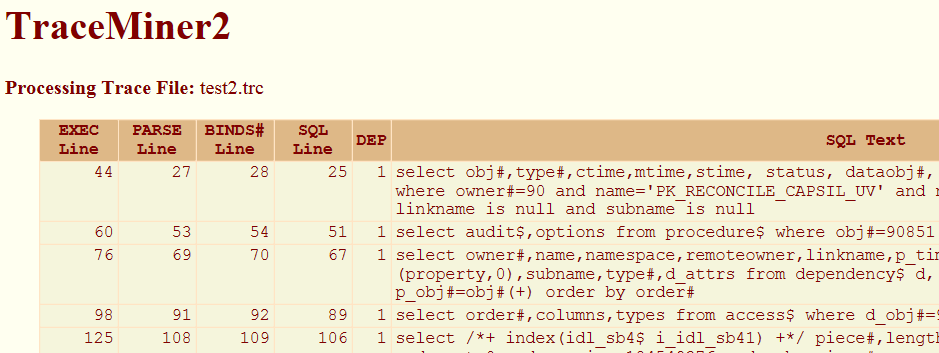
\includegraphics[width=\textwidth]{Content/images/TraceMiner2.png}

However, you can, if you have a standard report format at your company,
configure the generated css file to match that of your format.
\emph{TraceMiner2}\program{TraceMiner2} will not overwrite the css file if one exists in the
output folder.



\end{appendix}

\backmatter

%----------------------------------------------------------------------------------------
%	NDunbar: BIBLIOGRAPHY - NOT REQUIRED
%----------------------------------------------------------------------------------------

%\chapter*{Bibliography}
%\addcontentsline{toc}{chapter}{\textcolor{ocre}{Bibliography}}
%\section*{Books}
%\addcontentsline{toc}{section}{Books}
%\printbibliography[heading=bibempty,type=book]
%\section*{Articles}
%\addcontentsline{toc}{section}{Articles}
%\printbibliography[heading=bibempty,type=article]

%----------------------------------------------------------------------------------------
%	INDEX
%
% To make an index in MikeTex:
%
% Compile main file with pdfLaTeX.
% Compile main file with makeIndex -s StyleInd.ist.
% Compile main file with pdfLaTeX again.
%
%----------------------------------------------------------------------------------------

\cleardoublepage
\phantomsection
\setlength{\columnsep}{0.75cm}
\addcontentsline{toc}{chapter}{\textcolor{ocre}{Index}}
\printindex

%----------------------------------------------------------------------------------------

\end{document}
